%Input preamble
%Style
\documentclass[12pt]{article}
\usepackage[top=1in, bottom=1in, left=1in, right=1in]{geometry}
\parindent 22pt
\usepackage{fancyhdr}

%Packages
\usepackage{adjustbox}
\usepackage{amsmath}
\usepackage{amsfonts}
\usepackage{amssymb}
\usepackage{bm}
\usepackage[table]{xcolor}
\usepackage{tabu}
\usepackage{color,soul}
\usepackage{makecell}
\usepackage{longtable}
\usepackage{multirow}
\usepackage[normalem]{ulem}
\usepackage{etoolbox}
\usepackage{graphicx}
\usepackage{tabularx}
\usepackage{ragged2e}
\usepackage{booktabs}
\usepackage{caption}
\usepackage{fixltx2e}
\usepackage[para, flushleft]{threeparttablex}
\usepackage[capposition=top,objectset=centering]{floatrow}
\usepackage{subcaption}
\usepackage{pdfpages}
\usepackage{pdflscape}
\usepackage{natbib}
\usepackage{bibunits}
\definecolor{maroon}{HTML}{990012}
\usepackage[colorlinks=true,linkcolor=maroon,citecolor=maroon,urlcolor=maroon,anchorcolor=maroon]{hyperref}
\usepackage{marvosym}
\usepackage{makeidx}
\usepackage{tikz}
\usetikzlibrary{shapes}
\usepackage{setspace}
\usepackage{enumerate}
\usepackage{rotating}
\usepackage{tocloft}
\usepackage{epstopdf}
\usepackage[titletoc]{appendix}
\usepackage{framed}
\usepackage{comment}
\usepackage{xr}
\usepackage{titlesec}
\usepackage{footnote}
\usepackage{longtable}
\newlength{\tablewidth}
\setlength{\tablewidth}{9.3in}
\setcounter{secnumdepth}{4}

\titleformat{\paragraph}
{\normalfont\normalsize\bfseries}{\theparagraph}{1em}{}
\titlespacing*{\paragraph}
{0pt}{3.25ex plus 1ex minus .2ex}{1.5ex plus .2ex}
\makeatletter
\pretocmd\start@align
{%
  \let\everycr\CT@everycr
  \CT@start
}{}{}
\apptocmd{\endalign}{\CT@end}{}{}
\makeatother
%Watermark
\usepackage[printwatermark]{xwatermark}
\usepackage{lipsum}
\definecolor{lightgray}{RGB}{220,220,220}
%\newwatermark[allpages,color=lightgray,angle=45,scale=3,xpos=0,ypos=0]{Preliminary Draft}

%Further subsection level
\usepackage{titlesec}
\setcounter{secnumdepth}{4}
\titleformat{\paragraph}
{\normalfont\normalsize\bfseries}{\theparagraph}{1em}{}
\titlespacing*{\paragraph}
{0pt}{3.25ex plus 1ex minus .2ex}{1.5ex plus .2ex}

\setcounter{secnumdepth}{5}
\titleformat{\subparagraph}
{\normalfont\normalsize\bfseries}{\thesubparagraph}{1em}{}
\titlespacing*{\subparagraph}
{0pt}{3.25ex plus 1ex minus .2ex}{1.5ex plus .2ex}

%Functions
\DeclareMathOperator{\cov}{Cov}
\DeclareMathOperator{\corr}{Corr}
\DeclareMathOperator{\var}{Var}
\DeclareMathOperator{\plim}{plim}
\DeclareMathOperator*{\argmin}{arg\,min}
\DeclareMathOperator*{\argmax}{arg\,max}

%Math Environments
\newtheorem{theorem}{Theorem}
\newtheorem{claim}{Claim}
\newtheorem{condition}{Condition}
\renewcommand\thecondition{C--\arabic{condition}}
\newtheorem{algorithm}{Algorithm}
\newtheorem{assumption}{Assumption}
\renewcommand\theassumption{A--\arabic{assumption}}
\newtheorem{remark}{Remark}
\renewcommand\theremark{R--\arabic{remark}}
\newtheorem{definition}[theorem]{Definition}
\newtheorem{hypothesis}[theorem]{Hypothesis}
\newtheorem{property}[theorem]{Property}
\newtheorem{example}[theorem]{Example}
\newtheorem{result}[theorem]{Result}
\newenvironment{proof}{\textbf{Proof:}}{$\bullet$}

%Commands
\newcommand\independent{\protect\mathpalette{\protect\independenT}{\perp}}
\def\independenT#1#2{\mathrel{\rlap{$#1#2$}\mkern2mu{#1#2}}}
\newcommand{\overbar}[1]{\mkern 1.5mu\overline{\mkern-1.5mu#1\mkern-1.5mu}\mkern 1.5mu}
\newcommand{\equald}{\ensuremath{\overset{d}{=}}}
\captionsetup[table]{skip=10pt}
%\makeindex

\setlength\parindent{20pt}
\setlength{\parskip}{0pt}

\newcolumntype{L}[1]{>{\raggedright\let\newline\\\arraybackslash\hspace{0pt}}m{#1}}
\newcolumntype{C}[1]{>{\centering\let\newline\\\arraybackslash\hspace{0pt}}m{#1}}
\newcolumntype{R}[1]{>{\raggedleft\let\newline\\\arraybackslash\hspace{0pt}}m{#1}}



%Logo
%\AddToShipoutPictureBG{%
%  \AtPageUpperLeft{\raisebox{-\height}{
\includegraphics[width=1.5cm]{uchicago.png}}}
%}

\newcolumntype{L}[1]{>{\raggedright\let\newline\\\arraybackslash\hspace{0pt}}m{#1}}
\newcolumntype{C}[1]{>{\centering\let\newline\\\arraybackslash\hspace{0pt}}m{#1}}
\newcolumntype{R}[1]{>{\raggedleft\let\newline\\\arraybackslash\hspace{0pt}}m{#1}}

\newcommand{\mr}{\multirow}
\newcommand{\mc}{\multicolumn}

%\newcommand{\comment}[1]{}


\externaldocument{abccaretreatmenteffects_report_main_appendix}

\begin{document}
\title{\Large \textbf{Analyzing the Short and Long-term Effects of Early Childhood Education on Multiple Dimensions of Human Development}\thanks{This research was supported in part by the American Bar Foundation; the Pritzker Children's Initiative, the
Buffett Early Childhood Fund, NIH grants NICHD R37HD065072, NICHD R01HD54702, and NIA R24AG048081, an
anonymous funder, Successful Pathways from School to Work, an initiative of the University of Chicago's Committee
on Education funded by the Hymen Milgrom Supporting Organization, and the Human Capital and Economic
Opportunity Global Working Group, an initiative of the Center for the Economics of Human Development, affiliated with
the Becker Friedman Institute for Research in Economics, and funded by the Institute for New Economic Thinking. The
views expressed in this paper are solely those of the authors and do not necessarily represent those of the funders or
the official views of the National Institutes of Health. For helpful comments, we thank St\'{e}phane Bonhomme, Steven Durlauf, and Azeem Shaikh. For information on the implementation of the Carolina Abecedarian Project and assistance in data acquisition, we thank Peg Burchinal, Carrie Bynum, Frances Campbell, and Elizabeth Gunn. For information on childcare in North Carolina, we thank Richard Clifford and Sue Russell. For exceptional research assistance, we thank Thomas Choi. Lastly, we thank Sylvi Kuperman for sharing detailed and careful descriptions of the Carolina Abecedarian Project, as well as the federal and state childcare policies while the program was active. This information helped us improve estimates of the costs of the program and its alternatives.}}

\author{
Jorge Luis Garc\'{i}a\\
The University of Chicago \and
James J. Heckman \\
American Bar Foundation \\
The University of Chicago \and
Andr\'{e}s Hojman\\
The University of Chicago \and
Yu Kyung Koh \\ 
The University of Chicago \and
Joshua Shea \\
The University of Chicago \and
Anna Ziff \\ 
The University of Chicago}
\date{First Draft: January 5, 2016\\ This Draft: \today}
\maketitle

\singlespacing
%\pagebreak
\tableofcontents
\listoffigures
\listoftables
\pagebreak

\section{Introduction}

\noindent One of President Barack Obama's policy goals throughout his tenure has been the promotion of early childhood education as a means of reducing socio-economic inequality \citep{Bajaj_Labaton_2009_ObamaRiskAssets,White_House_2014_Econ_of_EC_Investments,White_House_2014_Fact_Sheet_Press}. Candidates across the political spectrum to succeed President Obama have also prioritized the discussion of early childhood education.\footnote{Candidates from both parties consider access to education a right Americans should have; all make particular emphasis on early childhood education \citep{Hillary-for-Am_2016_Universal-Preschool,On-the-Issues_2016_Sanders-on-Families,On-the-Issues_2016_Cruz-on-Education}.}\\ 

\noindent The relevance of early childhood education is not only a public debate matter. Public funding of early childhood education has been on the rise in recent years with the intention of reducing socio-economic inequality. The Education Commission of the States reports that 32 states increased spending on early childcare for the 2015-2016 year, with an overall state-spending increase of 12 percent. Similarly, the federal budget proposal for 2017 included an approximately \$300 million increase in spending on early childhood education.\\

\noindent Despite the importance of early childhood education both in the public debate and in the allocation of the government's budget, comprehensive and methodologically rigorous evidence on its efficiency and effectiveness  is still scarce. Many recent studies suffer from one of the following pitfalls: (i) they focus on a limited set of outcomes that fail to account for the complete set of program impacts;\footnote{An extreme example is the evaluation of preschool programs using an age-eligibility cutoff. A battery of studies compare children who were just eligible to children who were just ineligible given their birth dates and assess the gain of an additional year of preschool. This does not represent a comprehensive evaluation approach. Instead, it is an evaluation comparing an arbitrary set of children, in a very narrow set of tests. Examples of these studies include: \citet{Gormley_Gayer_2005_JHR,Gormley_Gayer_etal_2005_DP,Weiland_2013_CD_Impacts-of-Pre-K}.} (ii) they do not take into account that, even when evaluating randomized controlled trials, evaluation methodologies must account for randomization non-compliance and treatment substitution by the control families;\footnote{A relevant example is the evaluation of Head Start through its randomized controlled trial, the Head Start Impact Study \citep{Puma_Bell_etal_2010_HeadStartImpact}. Comparing the children in the treatment and the control groups usually yields relative low gains. This attenuation happens because a substantial proportion of children randomized out of the program were enrolled into preschool alternatives, some of them to other Head Start centers. Thus, a raw comparison between the treatment and the control groups children does not inform on either the efficiency or the effectiveness of Head Start. Studies providing a methodology to account for treatment substitution find that Head Start has substantial effects, although they focus on a single, short-term outcome \citep{Kline-Walters_2015_NBER-Evaluating,Feller_Grindal_etal_2016_ComparedtoWhat}.} or (iii) they evaluate randomized controlled trials with flawed designs.\footnote{An evaluation Tennessee Voluntary Prekindergarten is an emblematic example of this \citep{Lipsey_et_al_2013_Tennessee_Kindergrtn_PRI,Lipsey_et_al_2015_Randomized_Control_Trial_PRI}. The researchers designed a randomized controlled trial to evaluate the program. Unfortunately, they asked permission to assess the children after the randomization protocol. Thus, they have information available for children whose parents agreed for them to be evaluates \textit{post} randomization, inducing a potential imbalance between the children randomized in and out of the program. The evaluation does not account for that. Further, the results this evaluation present are on a narrow and short-term set of outcomes.}\\ 

\noindent  The case for the effectiveness and the economic efficiency of early childhood education in the U.S. is largely based on evidence from the Perry Preschool Program (referred to simply as Perry). Analyses of Perry suggests that (i) early childhood education has significant positive effects on multiple short and long-term socio-economic outcomes, even when accounting for compromised randomization, small-sample-size inference, and multiple hypotheses testing \citep{Heckman_Moon_etal_2010_QE}; (ii) early childhood education could have an annual internal rate of return that ranges between 7 and 10 percent;\footnote{If one dollar were to be invested at age 4, and then reinvested annually and compounded over a lifetime, the return would accrue to 60 to 300 dollars by age 65. This accounts for all the programs' cost and the social burden a government would cause by raising taxes to pay for it \citep{Heckman_Moon_etal_2010_RateofReturn}} and (iii) the mechanisms through which early education programs generate gains in long-term outcomes, namely that gains in socio-emotional skills---much more than gains cognitive skills---mediate decreases in criminal behavior and increases in employment and labor income \citep{Heckman_Pinto_etal_2013_PerryFactor}.\\

\noindent A frequent criticism of the evidence favoring the economic case for early childhood education is the lack of an ampler evidence base. In response, this paper presents a rigorous evaluation of two related randomized controlled trials: the Carolina Abecedarian Project (ABC) and the Carolina Approach to Responsive Education (CARE). These programs allow us to assess the short- and long-term effects of early childhood education on multiple dimensions of human development.\\

\noindent ABC and CARE were programs implemented in the early 1970s and late 1980s. Therefore, we observe long-term outcomes for their participants. The programs were separated into two phases. In the first phase, both programs assigned high-quality center-based childcare to children from ages 0 to 5. In addition, the children who were assigned center-based childcare in CARE also received home visits that aimed to foster the relationship between participating children and their parents. Further, CARE incorporated a second treatment group that received home visits without center-based childcare. The second phase of treatment, from ages 5 to 8, consisted of home visits that aimed to continue promoting childhood development. In ABC, the second stage treatment was randomly assigned independently of the first-phase randomization. The design of these programs allows us to tests hypotheses that evaluate the effectiveness of different type of programs, as well as the effectiveness of intervening at different stages of childhood.\\

\noindent As with any social experiment, the two programs pose methodological challenges. We construct a methodology to evaluate the program in the presence of these complications.\footnote{A usual critique to programs like ABC and CARE we do not assess here is their small sample size. Asymptotic inference methods, however, are well suited to analyze samples of the size of these programs \citep{Hanushek_Lindseth_2009_BOOKSchoolhousesCourthouses}. \citet{Campbell_Conti_etal_2014_EarlyChildhoodInvestments} evaluate the effectiveness of ABC at boosting health outcomes both using small sample size inference and an asymptotic procedure without finding little sensitivity if at all.}\\ 

\noindent We acknowledge and propose a methodology to account for cases of non-compliance to treatment, for which ABC has been criticized \citep{Hu_2014_ABC-Study}. Further, we present a thorough documentation for each of the cases of non-compliance for each stage of the data collection throughout both programs.\\ 

\noindent We also present a thorough documentation of control-group treatment substitution. In both programs, the parents of around 70\% of the children randomized out of center-based childcare enrolled their children in relatively high-quality preschool alternatives. We develop a methodology to account for treatment substitution and explain that there are two policy questions that we are able to ask using data from ABC and CARE. First, we can evaluate the effect of ABC and CARE given the supply of preschool alternatives available when they were implemented. Second, we can evaluate the effect of ABC and CARE relative to a fixed alternative: no preschool at all or a specified preschool alternative. The second question can better characterize the effectiveness of each program.\\

\noindent Finally, we propose a method to summarize the effectiveness of a program when information on multiple outcomes throughout the life-cycle is available. There are two current alternatives in the literature. One is to to calculate statistics that characterize the efficiency of a social program, such as the internal rate of return or the benefit-to-cost ratio \citep{Heckman_Moon_etal_2010_RateofReturn}. The other is to group outcomes into categories---e.g., cognition, criminal activity, health---and adjust the inference on each of the outcomes to account for multiple hypotheses testing and to avoid ``cherry picking'' significant results \citep{Lehman_Romano_2005_AnnStat,Lehmann_Romano_2005_testing,Heckman_Moon_etal_2010_QE}. In this paper, we propose a method to calculatie and formalize an inference procedure for (i) the count of outcomes for which the program causes a positive treatment effect; and (ii) the count of outcomes for which the program causes a \emph{significant} and positive treatment effect, considering different levels of significance.\footnote{This alternative is an application of conducting inference on a statistic that summarizes information across multiple sources---i.e., a combining function \citep{Pesarin_Salmaso_2010_PermutationTests}.}\\

\noindent \textbf{[JLG: next three paragraphs, description of results, pending.]}\\

\begin{comment}
\noindent In the rest of the paper, we formalize through several procedures the data description in Table~\ref{table:}, and find solid robustness \textbf{[MT: Unclear what this means...]}. We evaluate 141 outcomes describing human development throughout the life-cycle. Although we present counts over all the outcomes, we group them into categories for simplicity. These categories are maternal employment, life-cycle cognition, adolescent socio-emotional skills, adulthood socio-emotional skills, education, employment and income, crime, and health. For each outcome, we calculate the mean difference between the treatment and control groups in ABC and the treatment groups and the control group in CARE.\\

\noindent For ABC, 100 out of 141 outcomes indicate a positive treatment effects, as measured by the mean difference between the treatment and the control groups. When we limit the control sample to children who did not participate in any treatment alternatives, this number increases to 108. As we argue throughout the paper, this number more accurately describes the effectiveness of ABC because it compares treatment to a fixed, relative alternative: no treatment at all. Of the results, $54\%$ are positive and significant at the $10\%$ level. At the significance level of $10\%$, 14 outcomes should be positive and significant, a much lower number than $54\%$ \textbf{[MT: Something is wrong here, but I can't correct since the results have yet to be incorporated into the paper.]}.\\

\noindent For CARE, our findings indicate that the treatment incorporating center-based childcare \emph{and} home visits was much more effective than the treatment that had home visits only. These results are very much aligned with the results of ABC. Taken together, these comparisons establish that center-based childcare treatment is much more effective than home visits.\\
\end{comment}


\noindent We also test diverse hypotheses to assess the effectiveness of the second phase of randomization. The results are not at all comparable to the results of the first phase of randomization. We conclude that these programs were much more effective when intervening before age 5, rather than between ages 5 to 8.\\

\noindent This paper extends the work of \citet{Campbell_Conti_etal_2014_EarlyChildhoodInvestments}, who analyze the effectiveness of ABC at improving long-term health outcomes. It further presents the methodology and the treatment effect estimators that underpin our companion paper, \citet{Elango_et_al_2015_ABC_unpublished}. In it, we use the treatment effects in this paper to forecast the life-cycle gains of ABC on multiple dimensions of human development, from birth and until death, to calculate its internal rate of return and its benefit-to-cost ratio.\\

\noindent The rest of the paper proceeds as follows. Section~\ref{section:background} describes the background of each program. It includes an overview, a description of the eligibility criteria and the populations served, a characterization of the randomization protocol and of treatment substitution, and a comprehensive summary of the treatment.  Section~\ref{section:methodology} formalizes our methodology by discussing how we correct for compromised randomization and non-compliance, treatment substitution, and multiple hypotheses testing. Section~\ref{section:results} presents our main results and Section~\ref{section:conclusion} offers some final comments. An extensive appendix presents a much more thorough description of the program and data relative to what we present in the main text. It also discusses various alternative methodologies to evaluate the programs, and documents the results we present to a further extent.

\section{Background} \label{section:background}
\subsection{Overview}

\noindent The Carolina Abecedarian Project (ABC) and the Carolina Approach to Responsive Education (CARE) programs were designed and implemented by researchers at the Frank Porter Graham Center (FPGC) of the University of North Carolina in Chapel Hill. The programs targeted disadvantaged children from the semi-rural communities in the surrounding area.\\

\noindent The design and implementation of CARE and ABC were very similar. First, both studies had a small sample size. ABC recruited 122 children over four cohorts,\footnote{\citet{Ramey_Collier_etal_1976_CarolinaAbecedarianProject}.} while CARE recruited 65 children over two cohorts. Second, with respect to treatment, ABC had two phases, the first of which lasted from birth until the age of 5. In this phase, children were randomly assigned to either treatment or control groups. The treatment group received: (i) center-based childcare; (ii) breakfast, lunch, an afternoon snack, iron-fortified formula for the first 15 months of life, and a monthly supply of diapers; and (iii) medical care from licensed nurses who were supervised by a pediatrician, frequent health check-ups, and hospital referrals when serious medical treatment was needed. The control group only received formula and diapers. In the second phase of treatment, at the age of 5, the 95 children still in the study were randomly assigned again to treatment or control groups, independently of their status in the prior randomization. This treatment consisted of home visits targeting both children and parents and lasted until age 8.\\ 

\noindent  CARE also had two treatment stages, though children were randomized only once. While the two programs had essentially identical second stages, the first phase of CARE differed significantly from the first phase of ABC by including a family education component. This component was designed to study the effects of improving the home environment on child development.\footnote{\citet{Wasik_Ramey_etal_1990_CD}.} The first treatment phase of CARE lasted from birth until the age of 5. Children were randomly assigned to one of three experimental groups: control (23 children), family education (25 children), and both family education and center-based childcare (17 children). As in ABC, the control group received diapers and complementary nutrition from birth to 15 months. The family education group received home visits that aimed to help parents solve common problems related to childrearing. Both treatment groups received the second phase of treatment from ages 5 to 8.\\

\noindent The available data describing each program is rich and similar. In both programs, from birth until the age of 8, data was collected annually on cognitive and socio-emotional skills, home environment, family structure, and family economic characteristics. After age 8, the collection of data was less frequent. Information on cognitive and socio-emotional skills, education, and family economic characteristics was collected at ages 12, 15, 21, and 30.\footnote{At age 30, information on cognitive skills is unavailable for both ABC and CARE.} In addition, we have two sources of data that are novel to the program-evaluation literature: administrative criminal records and a full medical panel at age 34. These rich sources of data allow us to study the long-term effects of the programs on multiple aspects of human development.

\subsection{Eligibility Criteria and Populations Served} \label{section:eligibility}

\noindent ABC recruited four cohorts of children born between 1973 and 1977.\footnote{\citet{Feagans_1996_Childrens-Talk}.} CARE recruited two cohorts of children, one born in 1978 and one in 1979. The recruitment processes were identical. Potential families were referred to researchers by local social service agencies and hospitals at the beginning of the mother's last trimester of pregnancy. Eligibility was determined by a score of 11 in a High-risk Index (HRI).\footnote{The HRI was a linear combination based on 13 variables, which are listed here with their weights in parentheses: (i) maternal education level measured by years of education---6 (8), 7 (7), 8 (6), 9 (3), 10 (2), 11 (1), 12 (0); (ii) paternal education level with weights identical to those for maternal education; (iii) family income measured in current dollars---1,000 (8), 1,001-2000 (7), 2,001-3,000 (6), 3,001-4,000 (5), 4,001-5,000 (4), 5,001 (0); (iv) father's absence from the household for reasons other than health or death (3); (v) absence of maternal relatives in the area (3); (vi) siblings of school age one or more grades behind age-appropriate level, or with equivalently low scores on school-administered achievement tests (3); (vii) received payments from welfare agencies within past 3 years (3); (viii) record of father's work indicates instability or unskilled and semi-skilled labor (3); (ix) record of maternal or paternal IQ score of 90 or below (3); (x) record of sibling IQ score of 90 or below (3); (xi) relevant social agencies in the community indicate the family is in need of assistance (3); (xii) one or more family members has sought counseling or professional help in the past 3 years (1); and (xiii) special circumstances not included in any of the above that are likely contributors to cultural or social disadvantage (1).} Table~\ref{tab:baseline} compares the children in ABC and CARE. Overall, the children in CARE were relatively less disadvantaged; their mothers were older, more educated, and had higher IQ.

\begin{table}[H]
\captionsetup{singlelinecheck=false,justification=centering}
\caption{Baseline Characteristics Comparison between ABC and CARE \label{tab:baseline}}

  \begin{threeparttable}
  \begin{tabular}{cccccccc} \toprule

     &  & \scriptsize{ABC} & \scriptsize{CARE} & \scriptsize{ABC} & \scriptsize{CARE} & \mc{2}{c}{\scriptsize{$p$-value}} \\  

    \scriptsize{Variable} & \scriptsize{Age} & \scriptsize{Obs} & \scriptsize{Obs} & \scriptsize{Mean} & \scriptsize{Mean} & \scriptsize{Single $H_0$} & \scriptsize{Multiple $H_0$} \\ 
    \hline  

    \mc{1}{l}{\scriptsize{Male}} & \mc{1}{c}{\scriptsize{0}} & \mc{1}{c}{\scriptsize{116}} & \mc{1}{c}{\scriptsize{67}} & \mc{1}{c}{\scriptsize{0.464}} & \mc{1}{c}{\scriptsize{0.596}} & \mc{1}{c}{\scriptsize{\textbf{(0.060)}}} & \mc{1}{c}{\scriptsize{(0.110)}} \\  

    \mc{1}{l}{\scriptsize{Birth Weight}} & \mc{1}{c}{\scriptsize{0}} & \mc{1}{c}{\scriptsize{114}} & \mc{1}{c}{\scriptsize{64}} & \mc{1}{c}{\scriptsize{7.008}} & \mc{1}{c}{\scriptsize{7.139}} & \mc{1}{c}{\scriptsize{(0.625)}} & \mc{1}{c}{\scriptsize{(0.765)}} \\  

    \mc{1}{l}{\scriptsize{No. Siblings in Household}} & \mc{1}{c}{\scriptsize{0}} & \mc{1}{c}{\scriptsize{116}} & \mc{1}{c}{\scriptsize{67}} & \mc{1}{c}{\scriptsize{0.632}} & \mc{1}{c}{\scriptsize{0.684}} & \mc{1}{c}{\scriptsize{(0.810)}} & \mc{1}{c}{\scriptsize{(0.890)}} \\  

    \mc{1}{l}{\scriptsize{Birth Year}} & \mc{1}{c}{\scriptsize{0}} & \mc{1}{c}{\scriptsize{116}} & \mc{1}{c}{\scriptsize{67}} & \mc{1}{c}{\scriptsize{1974}} & \mc{1}{c}{\scriptsize{1979}} & \mc{1}{c}{\scriptsize{\textbf{(0.000)}}} & \mc{1}{c}{\scriptsize{\textbf{(0.000)}}} \\ 
    \midrule

    \mc{1}{l}{\scriptsize{Mother's Education}} & \mc{1}{c}{\scriptsize{0}} & \mc{1}{c}{\scriptsize{116}} & \mc{1}{c}{\scriptsize{67}} & \mc{1}{c}{\scriptsize{10.188}} & \mc{1}{c}{\scriptsize{10.868}} & \mc{1}{c}{\scriptsize{\textbf{(0.010)}}} & \mc{1}{c}{\scriptsize{\textbf{(0.025)}}} \\  

    \mc{1}{l}{\scriptsize{Mother's Age}} & \mc{1}{c}{\scriptsize{0}} & \mc{1}{c}{\scriptsize{116}} & \mc{1}{c}{\scriptsize{67}} & \mc{1}{c}{\scriptsize{19.828}} & \mc{1}{c}{\scriptsize{21.141}} & \mc{1}{c}{\scriptsize{\textbf{(0.060)}}} & \mc{1}{c}{\scriptsize{\textbf{(0.100)}}} \\  

    \mc{1}{l}{\scriptsize{Mother's IQ}} & \mc{1}{c}{\scriptsize{0}} & \mc{1}{c}{\scriptsize{116}} & \mc{1}{c}{\scriptsize{67}} & \mc{1}{c}{\scriptsize{84.407}} & \mc{1}{c}{\scriptsize{87.164}} & \mc{1}{c}{\scriptsize{\textbf{(0.070)}}} & \mc{1}{c}{\scriptsize{(0.130)}} \\  

    \mc{1}{l}{\scriptsize{Father at Home}} & \mc{1}{c}{\scriptsize{0}} & \mc{1}{c}{\scriptsize{116}} & \mc{1}{c}{\scriptsize{67}} & \mc{1}{c}{\scriptsize{0.283}} & \mc{1}{c}{\scriptsize{0.209}} & \mc{1}{c}{\scriptsize{(0.270)}} & \mc{1}{c}{\scriptsize{(0.380)}} \\  

  \bottomrule
  \end{tabular}
    \begin{tablenotes}
    \scriptsize
    \item 
    Note: This table compares baseline, observed characteristics between ABC and CARE. 
    For each characteristic, we present the $p$-value from a single hypothesis test.
    We also present the $p$-values from multiple testing, where we collectively test the
    baseline characteristics within the blocks separated by the horizontal line.
    Both $p$-values are two-sided and non-parametric. We construct them 
    based on 1,000 re-draws of the full sample. The estimates we display are the means of 
    the empirical bootstrap distribution. 
    
    \end{tablenotes}
  \end{threeparttable}

\end{table}

\noindent Neither ABC nor CARE used race as an eligibility factor. However, $98\%$ and $90\%$ of their participants were African-American, respectively.\footnote{\citet{Ramey_Smith_1977_AJMD,Ramey_Campbell_1984_AJMD,Ramey_Campbell_1991_childreninpoverty,Campbell_Pungello_etal_2001_DP}.} The average maternal age in ABC when the target child was born was 19.9, whereas in CARE mothers were on average 21 years old. In both treatments, approximately half of all mothers were 19 or younger.\footnote{Maternal age at target child's birth ranges from 13 to 43 years of age. One-third were 17 or younger.} Further, the average IQ for all mothers was 85 in ABC and 87 in CARE---approximately one standard deviation below the national mean. Only $25\%$ of the ABC children lived with both biological parents, and more than $50\%$ lived with extended families in multi-generational households ($61\%$ of treated children and $56\%$ of control children).\footnote{\citet{Ramey_Campbell_1991_childreninpoverty,Campbell_Ramey_1994_CD}.}\\

\begin{figure}[H]
\caption{Family Environment Baseline Characteristics, ABC and CARE}  \label{figure:baselineabccare}
    \centering
\begin{subfigure}{.5\textwidth}
  \centering
  \subcaption{Average Maternal Age}
  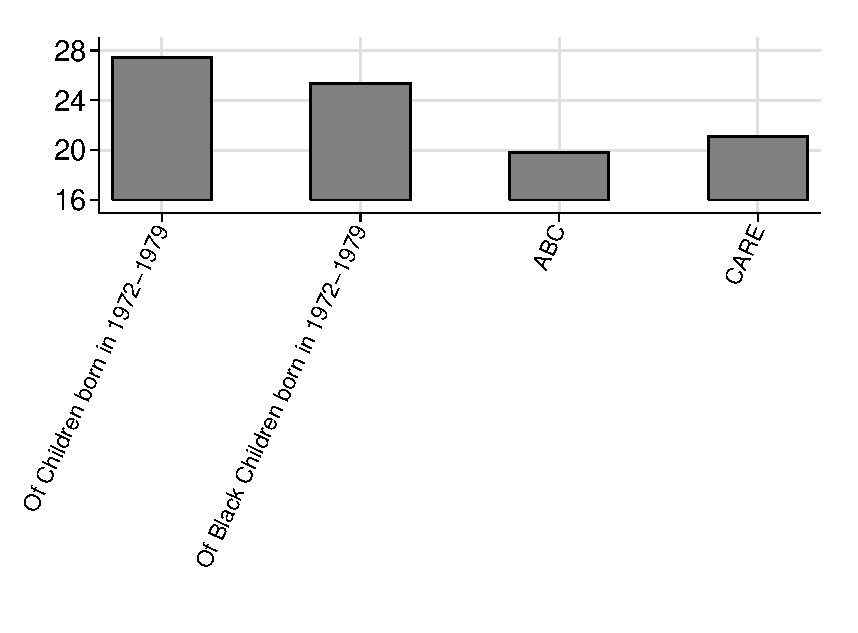
\includegraphics[height=2.3in]{output/abccarepsid_m_age0pool.eps}
\end{subfigure}%
\begin{subfigure}{.5\textwidth}
  \centering
  \subcaption{Average Maternal Years of Education} 
  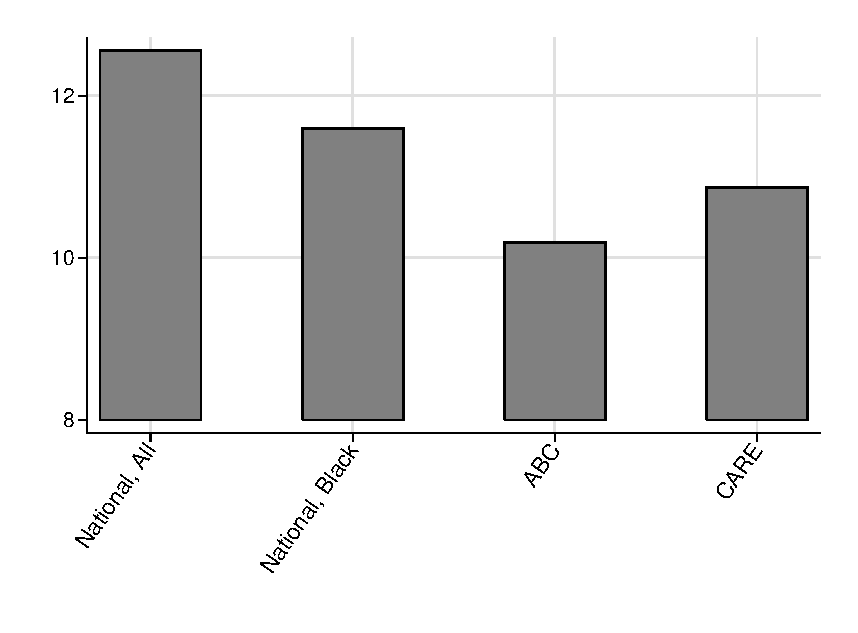
\includegraphics[height=2.3in]{output/abccarepsid_m_edu0pool.eps}
\end{subfigure}

\begin{subfigure}{.5\textwidth}
  \centering
  \subcaption{Proportion of Households with Father at Home}
  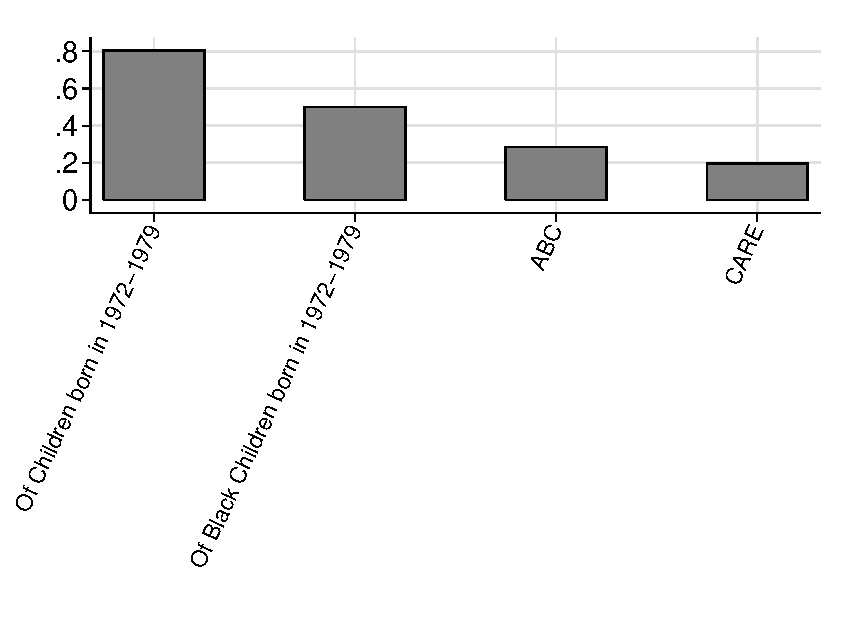
\includegraphics[height=2.3in]{output/abccarepsid_f_home0pool.eps}
\end{subfigure}%
\begin{subfigure}{.5\textwidth}
  \centering
  \subcaption{Median Parental Income in 1,000s of 2014 USD}
  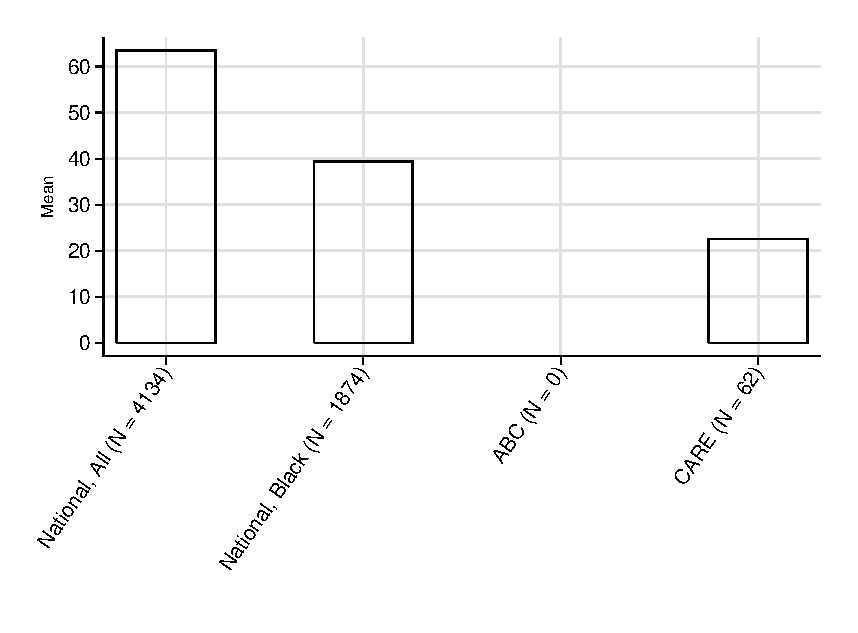
\includegraphics[height=2.3in]{output/abccarepsid_p_inc0pool.eps}
\end{subfigure}
\floatfoot{
\footnotesize
\noindent  Note: These panels plot four variable characteristics---mother's age, mother's education, an indicator of father at home, and parental income (in thousands of 2014 USD). In each panel, the first bar shows the national-level for a cohort born in the same years as the ABC and CARE individuals (1973-1979), obtained from the Panel Study of Income Dynamics (PSID). The second bar uses this same information restricted to black individuals. The third and fourth bars plot the same variables for ABC and CARE, pooling the treatment and control groups. We display the sample size for each calculation in parentheses next to the horizontal axis labels.
}
\end{figure}

\noindent To better characterize the socio-economic status of the families participating in ABC, we construct two comparison groups using the Panel Study of Income Dynamics (PSID), a nationally representative cohort of children born in the same years as the ABC and CARE participants (1973-1979), and a similar cohort restricted to black children. We show a comparison in Figure~\ref{figure:baselineabccare}. Compared to both nationally representative groups, ABC children were, on average, significantly more disadvantaged; they were born in households with extremely low total parental income and to younger, less educated mothers, most of whom were raising their children without the support of a father. The CARE participants were similarly disadvantaged compared to nationally representative groups with respect to these basic household socio-demographic characteristics.\\

\subsection{Randomization Protocol and Compromises} \label{section:randomization}

\subsubsection{ABC}

\noindent The first phase of randomization was conducted at the family level, so pairs of siblings and twins were jointly randomized to either treatment or control groups.\footnote{Sibling pairs occurred when the two siblings were close enough in age such that both of them were eligible for the program.} Although we know that the pairing was based on HRI, maternal characteristics, number of siblings, and gender, we do not knows the original pairs. Overall, the study comprised 120 families. As discussed below, our calculations indicate that 112 families participated in the initial randomization, while 8 families became part of the program as replacement for the families that withdrew.\\

\noindent There were some compromises in the first phase of randomization. One control child participated in the program, as any other child of the treatment group and three children in the treatment group did not participate, due to the decisions of their families. We have information on these children and their families from birth until the end of elementary school. Four families moved out of the area before any data on them was collected and only data from adulthood is available. Two children in the control group were swapped into treatment at the request of local authorities, because they were considered to be at high-risk of developmental delay. Two additional children in the control group were dropped because they were diagnosed with a developmental delay, which made them ineligible for the program. Most of the data for these last four control children is available from birth until elementary school. Finally, four children died before age 5.\footnote{One child in the control group died at 3 months from cardiomyopathy and seizure disorder, and a second child in the control group died at 18 months from a cardiac arrest. One child in the treatment group died at 3 months from crib death, while the other died in a pedestrian accident at 50 months \citet{Ramey_Campbell_1984_AJMD}.} Thus, we classify 14 children as cases of attrition.

\noindent The children who stopped participating in the program before they were 6 months old were found replacements with comparable observed characteristics.\footnote{Three replacements are documented in \citet{Ramey_Campbell_1979_SR}. One is documented in correspondence with the program officers, which is available from the authors of this document upon request. The rest are implied by the number of children who participated of the randomization in each cohort.} Overall, the first phase sample consisted of 111 children: 53 treatment children and 58 control children.\\

\noindent Prior to the second phase of randomization, 3 children in the control group of the first phase and 3 children in the treatment group of the first phase stopped being followed because it was impossible to find them. One child in the control group and 8 children in the treatment group of the first phase did not participate in the second phase but later agreed to participate in the data collections during adulthood. This yielded a sample of 96 children in the second phase: 49 in treatment and 47 in control. After randomization, three children in the treatment group chose not to participate in the program, while all children in the control group adhered to their randomization status. Figure~\ref{fig:abc-flow} illustrates the randomization protocol for the two phases of the program.

\newgeometry{top=.8in, bottom=.8in, left=1in, right=1in}

\begin{center}
	\begin{figure}[H]
		\caption{Randomization Protocol and Treatment Compliance, ABC} \label{fig:abc-flow}
		\centering
		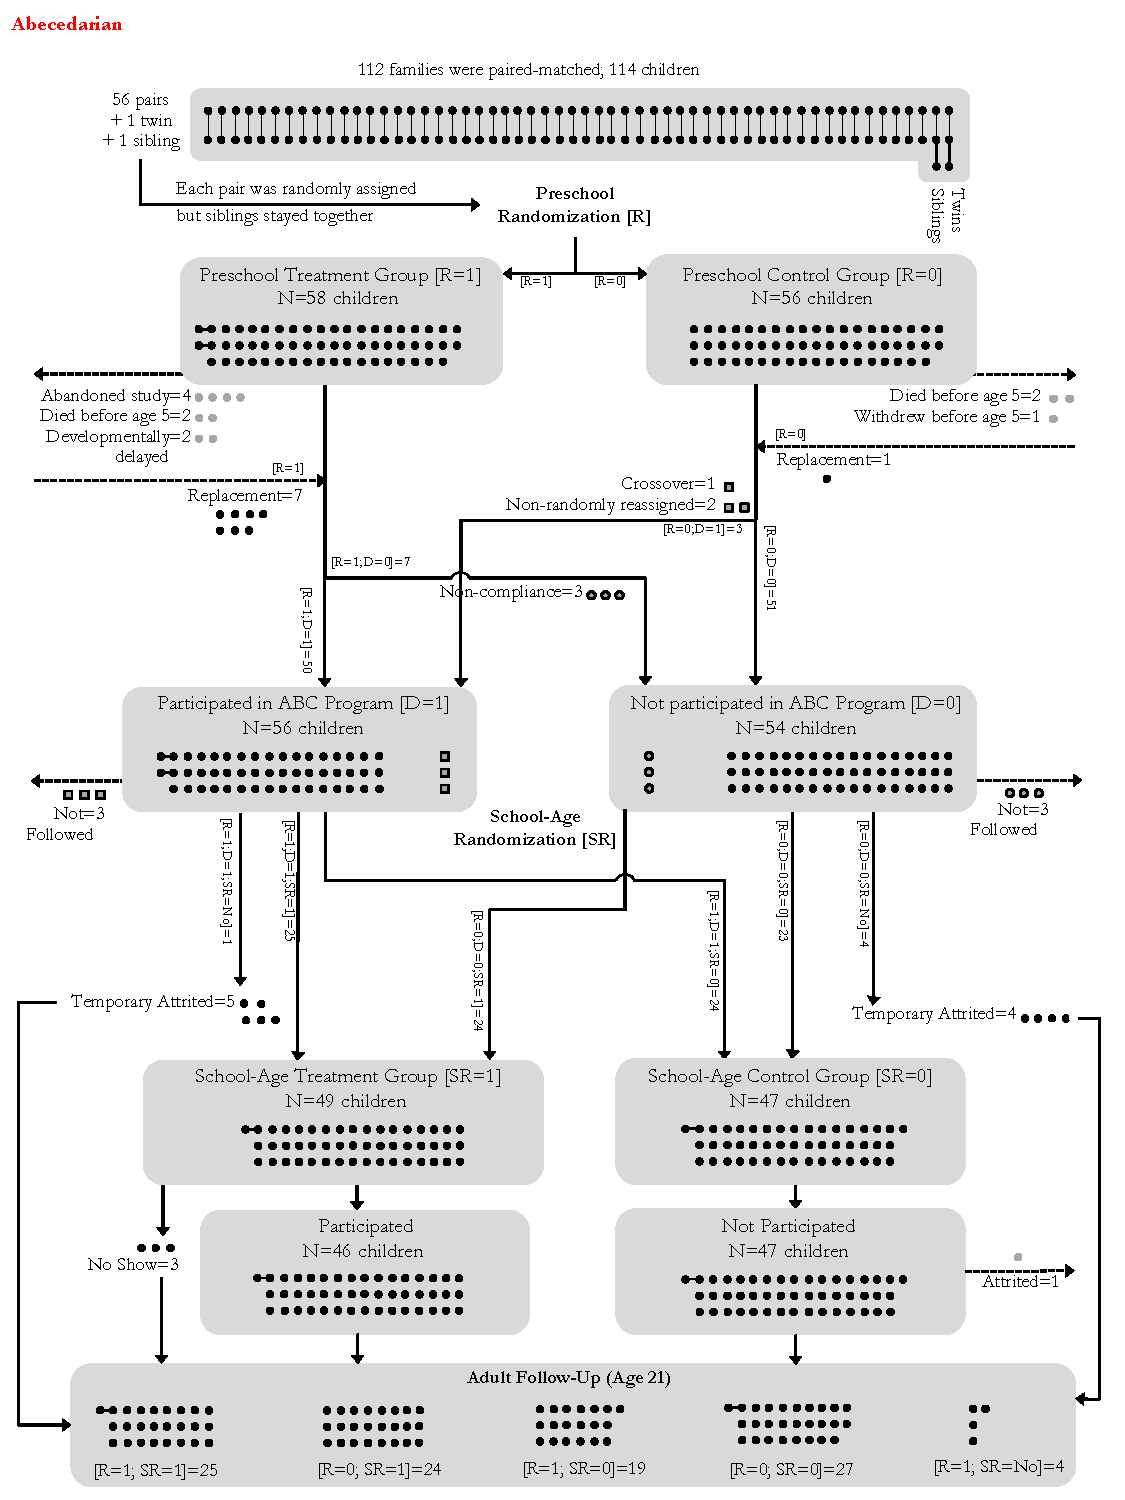
\includegraphics[width=.83\columnwidth]{output/abc_Diagram.pdf}
\floatfoot{
\footnotesize
\noindent
Sources: \cite{Ramey_Collier_etal_1976_CarolinaAbecedarianProject, Ramey_Smith_1977_AJMD,Ramey_Campbell_1979_SR,Ramey_Campbell_1984_AJMD}, internal documentation of the program, and own calculations. Note: The variable R represents randomization into treatment [R=1] or control [R=0]. After the original randomization, some children died or withdrew from the program early in life and were replaced. R also includes those replacements. Arrows pointing outside the diagram indicate children who left the study permanently. The variable P represents participation in the preschool-age program. The variable SR represents randomization into the school-age program [SR=1], or out of it [SR=0]. Some children were not randomized at school age [SR=No]. We use the term temporary attrited for children who did not participate in the study at school age, but were later interviewed in the age-21 followup.
}
	\end{figure}
\end{center}

\restoregeometry

\noindent The compromises to randomization pose a methodological challenge that we address when calculating the effects the program on all outcomes and across all ages for which we have data. We develop our methodology further in Section~\ref{section:methodology}.\footnote{In Appendix~\ref{appendix:randomization} we show various comparison exercises to assess how the randomization compromises affect the balance between the treatment and control groups. In sum, we find that the various randomization compromises do not affect the balance in baseline, observed characteristics.}

\subsubsection{CARE}

\noindent 
The randomization protocol in CARE was analogous to the first phase of randomization in ABC. Notably, it had no major compromises.\footnote{\citet{Bryant_et_al_1987_Carolina_Approach_TIECSE,Wasik_Ramey_etal_1990_CD,Burchinal_Campbell_etal_1997_CD}.} Of the 65 initial families, 23 were randomized to control, 25 to the family education treatment group, and 17 to the family education and center-based childcare treatment group. Two families in the family education treatment group had twins who were jointly randomized, as in ABC. After randomization, the family of one child initially assigned to the family education and center-based childcare treatment refused its status and did not participate in the program. Within the first six months of treatment, one child assigned to this same group left the study due to family relocation. Finally, one child who was assigned to the family education treatment group died. Figure~\ref{fig:care-flow} illustrates CARE's randomization and the flow of participants throughout the data follow-ups.\\

\begin{center}
	\begin{figure}[H]
		\caption{Follow-up Availability and Attrition, CARE} \label{fig:care-flow}
		\centering
		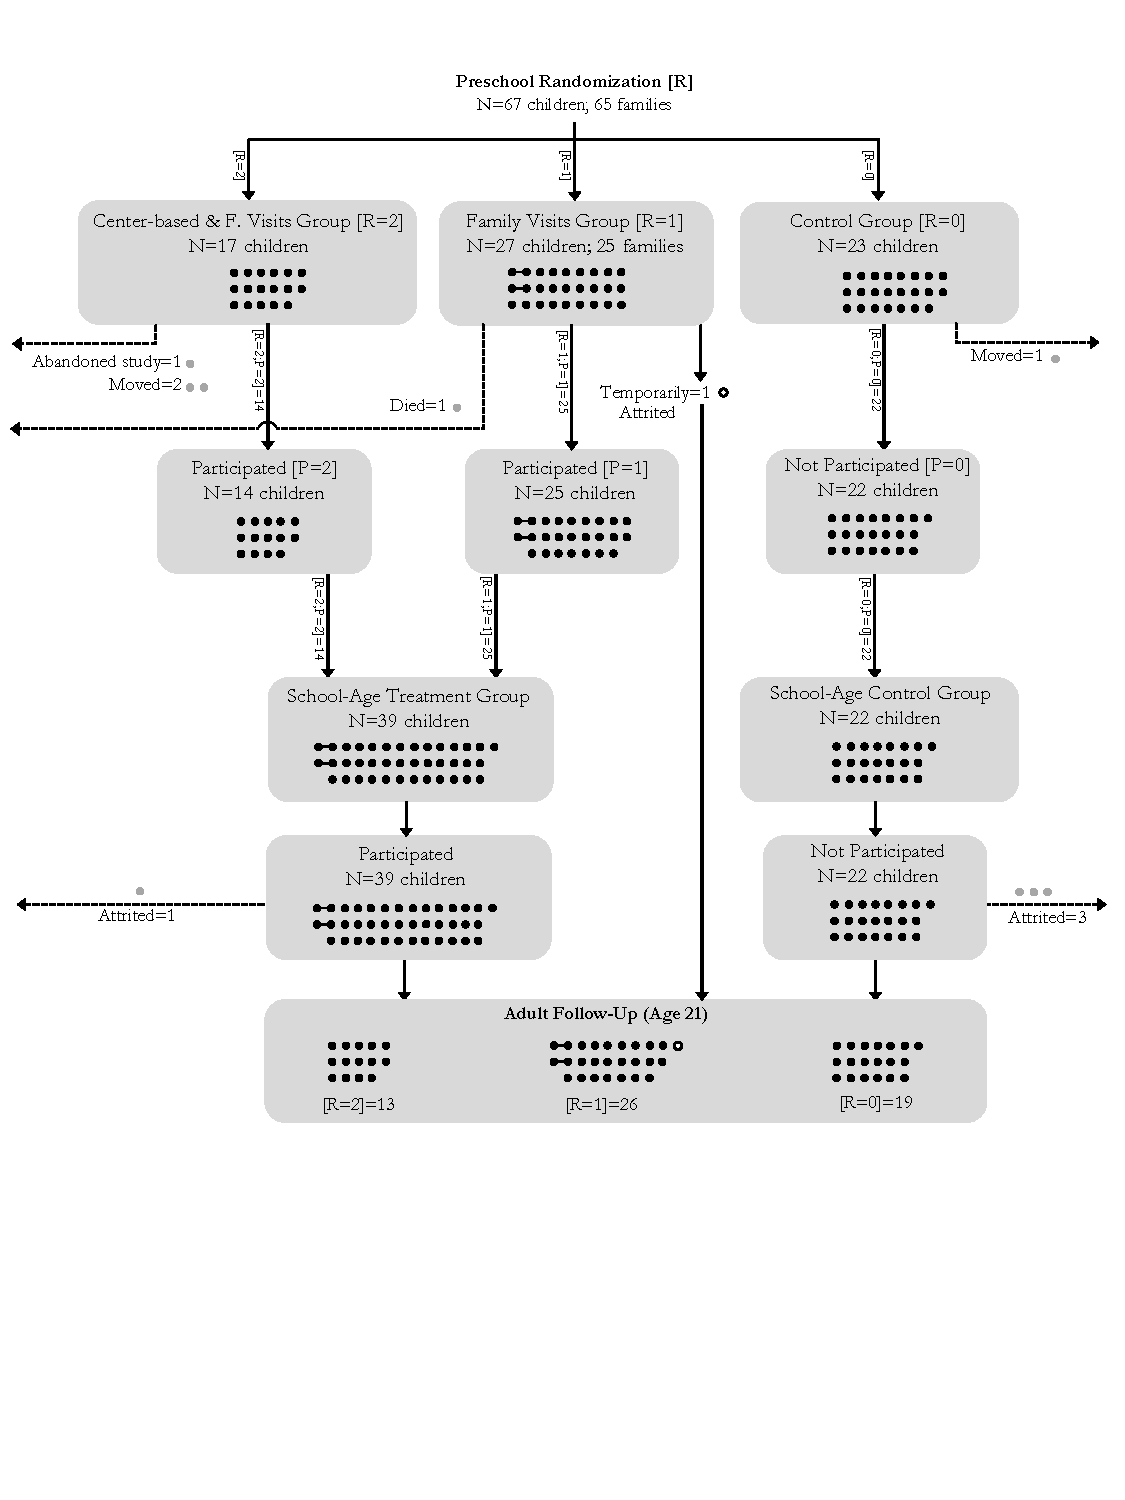
\includegraphics[width=.9\columnwidth]{output/care_Diagram.pdf}
\floatfoot{
\footnotesize
\noindent 
Sources: \cite{Wasik_Ramey_etal_1990_CD}, internal documentation of the program, and own calculations. Note: The variable R represents randomization into control [R=0], family education treatment [R=1], and family education and center-based childcare treatment [R=2]. Arrows pointing outside the diagram indicate children that left the study permanently. The variable P represents participation in the respective programs. Both the treatment groups continued into school-age with a home visitation program that was not randomized. We use the term temporarily attrited for children who did not participate in the study at school age, but were interviewed in the age-21 followup.}
	\end{figure}
\end{center}

\subsection{Program Description and Content}

\noindent The ABC and CARE programs shared many objectives and program characteristics, as summarized in Table~\ref{tab:programcomparison}.\\

\begin{table}[H]
\begin{center}
\begin{threeparttable}
\caption{ABC and CARE, Programs Comparison} \label{tab:programcomparison}
\scriptsize
\scalebox{.9}{\begin{tabular}{L{4cm} L{7cm} L{5cm}}
\hline \hline
& \multicolumn{1}{c}{ABC}& \multicolumn{1}{c}{CARE}\\
\hline 
Program Overview &&\\
\hspace{.5cm} Years Implemented &1972--1982&1978--1985\\
\hspace{.5cm} Age of Entry/Exit & birth to 5 years old &\checkmark\\
\hspace{.5cm} Initial Sample &122&64\\
\hspace{.5cm} \# of Cohorts &4&2\\
\midrule
Eligibility & socio-economic disadvantage according to a multi-factor index (see Section \ref{section:eligibility})&\checkmark\\
 \midrule
Control &&\\
\hspace{.5cm} N &54&23\\
\hspace{.5cm} Compensation & Diapers from birth to age 3, unlimited formula from birth to 15 months & \checkmark \\
\hspace{.5cm} Treatment Substitution & 70\% & $\sim$ 70\%\\
\midrule
Treatment & Center-based childcare & Center-based childcare and family education\\
\hspace{.5cm} \textbf{Center-base} &&\\
\hspace{.5cm} \textbf{Childcare} &&\\
\hspace{.5cm} N &57&17\\
\hspace{.5cm} Intensity &6.5--9.75 hours a day for 50 weeks per year&\checkmark\\
\hspace{.5cm} Components & Instruction, medical care, nutrition, social services &\checkmark\\
\hspace{.5cm} Staff-to-child Ratio &1:3 during ages 0--1 &\checkmark\\
&1:4--5 during age 1--4 &\checkmark\\&1:5--6 during ages 4--5 &\checkmark\\
\hspace{.5cm} Staff Qualifications &Mixed diplomas; experienced&\checkmark\\
\hspace{.5cm} \textbf{Family Education} & Not part of the program &24\\
\hspace{.5cm} Intensity && One hour-long home visits. 2--3 per month during ages 0--3. 1--2 per month during ages 4--5\\
\hspace{.5cm} Curriculum & & Social and mental stimulation; parent-child interaction\\
\hspace{.5cm} Staff-to-child Ratio &&1:1\\
\hspace{.5cm} Staff Qualifications &&Home visitor training\\
\midrule
 School-age Treatment \\
 \hspace{.5cm} N&46&39\\
\hspace{.5cm} Intensity &Every other week& \checkmark\\
\hspace{.5cm} Components &Parent-teacher meetings& \checkmark\\
\hspace{.5cm} Curriculum & Reading and math &\checkmark\\
\hspace{.5cm} Staff-to-child Ratio &1:1&\checkmark\\
\hspace{.5cm} Staff Qualifications &Graduate degree and training in special education & \checkmark\\
\midrule
Data Availability \\
Questionnaires & Ages 0--5, 8, 12, 15, 21, 30--34 & Ages 0--5, 8, 12, 21, 30--34 \\
Parent Interview & Ages 0--5, 8, 12, 15, 21& Ages 0--5, 9, 12 \\  
Health Follow-up & Ages 30--34&\checkmark\\
\hline \hline
\end{tabular}}
\footnotesize
\begin{tablenotes}
\item Note: This table compares the main elements of ABC and CARE, summarized within this section.
\end{tablenotes}
\end{threeparttable}
\end{center}
\end{table}

\noindent ABC and CARE shared a main objective: to prevent ``mental retardation" and to develop school readiness for disadvantaged children, starting at birth.\footnote{Note that the clinical understanding of mental retardation was once associated with disadvantages that hindered early-life development \citep{Mental-Retardation_America_2004_BOOK_NYU}.} The different curricula implemented iacross programs and cohorts had the following common goals: (i) to support language and cognitive development; and (ii) to develop socio-emotional competencies that were considered to enable school readiness---e.g. task orientation, emotional self-expression, independence, sharing, and cooperation.\footnote{\citet{Sparling_1974_Synth_Edu_Infant_SPEECH,Ramey_Collier_etal_1976_CarolinaAbecedarianProject,Ramey-etal_2012-ABC}.} The curricula evolved each year according to recommendations made in studies that used the children's data.\footnote{\citet{Ramey-etal_1975_AJoMD,Finkelstein_1982_Day_Care_YC,Haskins_1985_CD}.}$^{,}$\footnote{The curricula implemented in the first phases of ABC and CARE, including Tools of Mind, shared an emphasis on self regulation---e.g., goal setting and self-reflection---and opportunities for language development. Language development, including phonics and reading skills, is also an important element in other widely implemented curricula such as Opening the World of Learning.}$^{,}$\footnote{Two other renowned early childhood education programs are worth comparing to ABC and CARE. The Infant Health and Development Project (IHDP) was based on the first phase of CARE. IHDP had a single treatment group, which was very similar to the center-based childcare and family education treatment group of CARE. The curricula implemented both at home and at center-based childcare were very similar. The main difference is that the first phase of CARE lasted 5 years, while IHDP lasted 3 years and did not have a second phase. Both ABC and CARE were notably different from the Nurse Family Partnership (NFP) program. NFP had fewer visits and began in the pre-natal period. Mothers received monthly visits during pregnancy and one visit every two months from when the child was born until the age of 2. The visitors were nurses and they tried to help women build relationships with friends and family to create a support network for their children. A common element of the three programs is that the visitors helped parents use community resources when solving their everyday problems.}\\

\noindent Both treatment groups in CARE incorporated home visits, which aimed to help parents resolve everyday problems that could adversely affect relationships with their children, as well as to improve the general skills associated with parenting. Generally, the home visits were weekly and one hour long. Between birth and the age of 3, participants in the family education and center-based childcare and family education groups received, on average, 2.5 and 2.7 visits a month, respectively. At ages 4 and 5, the average frequency decreased to 1.4 and 1.1 visits per month.\\ 

\noindent The first phases of ABC and CARE were conducted in conjunction with a longitudinal medical research study on infectious respiratory diseases in group environments.\footnote{\citet{Henderson-et-al_1982_NEJoM}.} This study allowed the children to have comprehensive medical care in the same center in which they received center-based childcare. The children who attended the center received daily screenings to detect any signs of illness. This included all the children in the treatment group of ABC and all the children in the center-based childcare and family education group of CARE. The first cohort of the control group of ABC also received frequent medical check-ups during the first year of the first-phase of the program.\\

\noindent The children assigned to treatment in the first phase of ABC also received primary pediatric care by a family nurse practitioner and a licensed practical nurse, who were supervised by a pediatrician who was on continuous duty at the center-based childcare center. This care consisted of wellness check-ups, immunizations, parental counseling, and initial assessments of illnesses. Like the other treatment components, pediatric care was free of charge. Unfortunately, there is no documentation or corresponding evidence for whether this aspect of treatment was available to the treatment groups of CARE.\\

\noindent For both ABC and CARE, children in the programs' center-based childcare were provided breakfast, lunch, and an afternoon snack, planned by a nutritionist. Children in the control groups of both programs received diapers from birth until the age of 3, and an unlimited supply of bottled formula from birth until 15 months. Neither control group nor CARE's family education treatment group received any program medical care, with the exception of the first cohort of control children in ABC, as explained above.\\

\noindent The second phase of CARE, also referred to as school-age treatment, lasted for the first three years of elementary school and incorporated home visits by a teacher. The visits aimed to increase the child's exposure to reading and mathematics and to promote parental involvement in the learning process. These visits occurred every two weeks in the presence of the parents. At the visits, the teachers discussed the children's programs and helped parents with issues related to literacy, housing, and medical care.\\

\subsection{Treatment Substitution}

\noindent The interpretation of treatment and control group comparisons depends on how the control group substituted for treatment, posing a methodological challenge when answering policy-oriented questions. In both programs, many children without access to center-based childcare through random assignment nevertheless attended alternative preschools. In this section, we characterize the types of care received by the treatment group. We propose a methodology to answer relevant policy-questions in Section~\ref{section:methodology}.\\

\begin{figure}[H]
		\caption{Treatment Substitution, ABC} \label{fig:treatsubabc}
		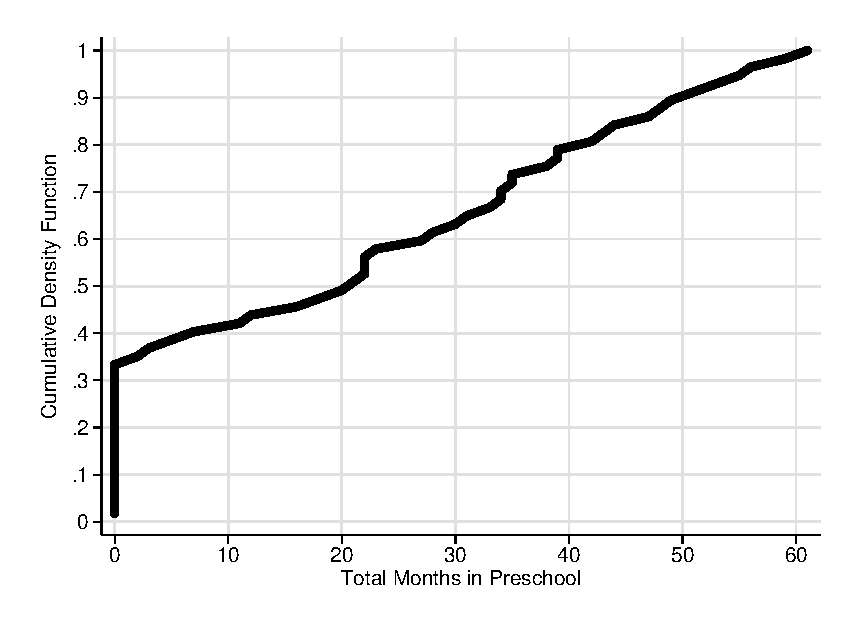
\includegraphics[width=.9\columnwidth]{output/abc_controlcontamination_months.eps}
\floatfoot{
\footnotesize
\noindent Note: This figure displays the cumulative density function of enrollment in an alternative preschool for the control group in ABC.}
\end{figure}

\noindent In ABC, $70\%$ of control-group children was enrolled in one of 11 local center-based childcare centers (see Figure~\ref{fig:treatsubabc}). Each of these centers received federal subsidies and were therefore regulated by the Federal Interagency of Daycare Requirements. Therefore, their staff members were required to be trained in early childhood education and the centers were required to implement approved curricula designed to enhance cognitive, social, and linguistic competence in disadvantaged children.\footnote{\citet{Burchinal_etal_1989_CD_Daycare-Pre-K-Dev}.} In CARE, slightly more than $70\%$ of the control group and $60\%$ of the family education group were enrolled in alternative preschools by their parents (see Figure~\ref{fig:treatsubcare}). The parents of the children in both of these groups had as options the same set of local center-based childcare centers as the ABC children in the control group.

\begin{figure}[H]
		\caption{Treatment Substitution, CARE} \label{fig:treatsubcare}
		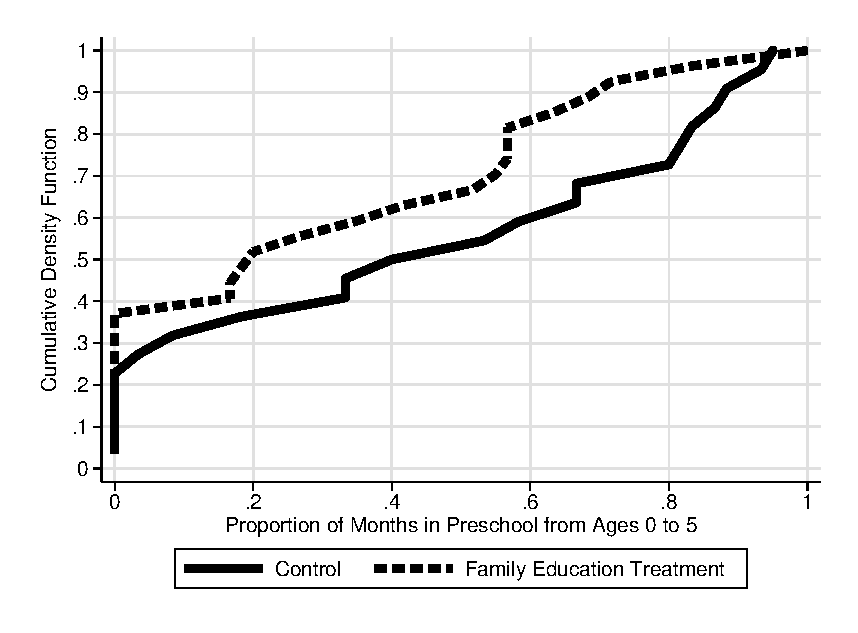
\includegraphics[width=.9\columnwidth]{output/care_controlcontamination_months.eps}
\floatfoot{
\footnotesize
\noindent Note: This figure displays the cumulative density function of enrollment in an alternative preschool for the control and family education treatment groups in CARE.}
\end{figure}
 

\subsection{Data} \label{section:data}

\noindent In Table~\ref{tab:ecvars_1} to Table~\ref{tab:adultvars_2}, we summarize the data availability for both ABC and CARE. The data collection processes in both programs were analogous by design. For both programs, the treatment and control groups were followed into adulthood with relatively low attrition. For ABC, children were followed annually through elementary school and at ages 12, 15, 21, and 30. Health and administrative crime data were collected when the children reached their mid-30s. For CARE, the exact same follow-ups are available with the exception of the age 15 follow-up.\\

\begin{sidewaystable}[H]
\small
\caption{Early Childhood Data (Part I)}
\label{tab:ecvars_1}
\centering
\begin{adjustbox}{max width=\textwidth, max height=\textheight,keepaspectratio}
\begin{threeparttable}
\tiny
\begin{tabular}{L{3cm} C{3.5cm} C{4cm} C{1.5cm} C{1.5cm}  C{6cm}}
\toprule
\textbf{Category}	&	\textbf{Sub-Category}	&	\textbf{Description}	&	\textbf{ABC Age}  	&  \textbf{CARE Age}  & 	\textbf{Measure}	\\ \midrule
Demographics	&	Gender	&	Gender of child	&	Birth, 18, 30, 42, 54	&	 Birth, 18, 30, 42, 54	&	Demographic Interview	\\
	&	\\
	&	Race	&	Race/Cultural identity of child	&	Birth, 18, 30, 42, 54	&	 Birth, 18, 30, 42, 54	&	 Demographic Interview\\
	&	\\
	&	Birth Date	&	Date of birth of child	&	Birth, 18, 30, 42, 54	& 	Birth, 18, 30, 42, 54	&	 Demographic Interview	\\ \midrule
Cognitive Assessments	&	Language Ability	&	Auditory association, Verbal expression, etc. 	&	36, 42, 48, 54	&	30, 42, 54	&	ITPA$^{ABC}$, GPB$^{ABC}$, PLP$^{ABC}$, MSCD \\
	&	\\
	&	Intelligence Levels	&	SBIS 	&	24, 36, 48, 60	&	24, 36, 48, 60	&	SBIS	\\
	&		&	WPPSI	&	60	&	60	&	WPPSI	\\
	&		&	BSID 	&	3, 6, 9, 12, 18, 24	&	6, 12, 18, 24		&	BSID	\\
	&		&	UOSPD	&	15	&	- 	&	UOSPD$^{ABC}$	\\
	&		&	RPM	&	60	&	-	&	RPM$^{ABC}$	\\
	&	\\
	&	Quantitative	 &	BSID 	&	3, 6, 9, 12, 18, 24	&	6, 12, 18, 24		&	BSID	\\
	&		&	MSCD 	&	30, 42, 54		&	30, 42, 54	&	MSCD	\\
	&	\\
	&	Memory	&	BSID 	&	3, 6, 9, 12, 18, 24	& 	6, 12, 18, 24		&	BSID	\\
	&		&	MSCD 	&	30, 42, 54	&	30, 42, 54	&	MSCD	\\
	&	\\
	&	Motor Development	&	BSID 	&	3, 6, 9, 12, 18, 24	&	6, 12, 18, 24		&	BSID\\
	&		&	MSCD 	&	30, 42, 54	&	30, 42, 54	&	MSCD	\\
	& 	\\
	&	Critical Thinking	&	Curiosity	&	30, 36, 42, 48, 54, 60, 66, 72	& - &	Infant Behavior Inventory$^{ABC}$	\\ \midrule
Non-Cognitive Assessments	&	Social Skills	&	Positive social response	&	30, 36, 42, 48, 54, 60, 66, 72	&	6, 12, 18, 24		&	Infant Behavior Inventory$^{ABC}$, Bayley Infant Inventory$^{CARE}$	\\
	&		&	Creativity	&	30, 36, 42, 48, 54, 60, 66, 72	&	- 	&	Infant Behavior Inventory$^{ABC}$	\\
	&	\\
	&	Self-Control	&	Locus of control	&	3, 18	&	6, 18	& 	RIES	\\
	&		&	Distractibility, Attentiveness	&	30, 36, 42, 48, 54, 60, 66, 72	&	6, 12, 18, 24		&	Infant Behavior Inventory$^{ABC}$, Bayley Infant Inventory$^{CARE}$	\\
	&	\\
	&	Emotional Health	&	KRT	&	24, 36, 48, 60	&	24, 30, 36, 42, 48, 60	&	KRT	\\
	&	\\
	&	Self-Consciousness	&	Self-consciousness	&	30, 36, 42, 48, 54, 60, 66, 72	&	-	&	Infant Behavior Inventory$^{ABC}$	\\
\bottomrule
\end{tabular}
\begin{tablenotes}
\scriptsize
\item Sources: Authors' description. \\	
\item Note: This table describes the major categories of variables that were measured for ABC and CARE subjects up to age 6. ABC and CARE ages are measured in months. This is not an exhaustive list of variables, nor does it include variables from auxiliary data. Instruments or questionnaires available for only one of the studies are indicated with the superscript $^{ABC}$ or $^{CARE}$.  \textbf{Abbreviations are as follows.} ITPA: Illinois Test of Psycholinguistic Ability. GPB: Gordon Psycholinguistic Battery. PLP: Preschool Language Performance. MSCD: McCarthy Scales of Children's Development. BSID: Bayley Scales of Infant Development and Infant Behavior. UOSPD: Uzgiris-Hunt Ordinal Scales of Psychological Development. RPM: Raven's Progressive Matrices. RIES: Rotter's Internality-Externality Scale. KRT: Kohn and Rosman Test Behavior Inventory.
\end{tablenotes}
\end{threeparttable}
\end{adjustbox}
\end{sidewaystable}




\begin{sidewaystable}[H]
\small
\caption{Early Childhood Data (Part II)}
\label{tab:ecvars_2}
\centering
\begin{adjustbox}{max width=\textwidth, max height=\textheight,keepaspectratio}
\begin{threeparttable}
\tiny
\begin{tabular}{L{3cm} C{3.5cm} C{4cm} C{1.5cm} C{1.5cm}  C{6cm}}
\toprule
\textbf{Category}	&	\textbf{Sub-Category}	&	\textbf{Description}	&	\textbf{ABC Age}  	&  \textbf{CARE Age}  & 	\textbf{Measure}	\\ \midrule
Family Environment	&	Family Members	&	Number of primary caretakers	&	Birth, 18, 30, 42, 54	&	18, 30, 42, 54, 60	&	Demographic Interview	\\
	&		&	Relationship with family members, including father, mother, siblings, etc.	&	Birth, 18, 30, 42, 54	&	18, 30, 42, 54, 60	&	Demographic Interview	\\
	&		&	Number of siblings	&	Birth, 18, 30, 42, 54	&	Birth, 18, 30, 42, 54, 60	&	Demographic Interview	\\
	&		&	Marital status of parents	&	Birth, 18, 30, 42, 54	&	Birth, 18, 30, 42, 54, 60	&	Demographic Interview	\\
	&		&	Marital conflicts between parents	&	6, 18	&	Birth, 6, 18, 36	&	Demographic Interview$^{CARE}$, Parental Attitudes Research Inventory	\\
	&		& Father at home & 18, 30, 42, 54  & 18, 30, 42, 54, 60 & Demographic Interview \\
	&	\\
	&	Family Economic Environment	&	Parents' occupation	&	Birth, 18, 30, 42, 54	& 	Birth, 18, 30, 42, 54, 60		&	Demographic Interview	\\
	&								& Mother works & 18, 30, 42, 54 & 18, 30, 42, 54, 60 & Demographic Interview \\
	&		&	Source of child support	&	Birth, 18, 30, 42, 54	&	18, 30, 42, 54, 60	&	Demographic Interview	\\
	&		&	Family income	&	Birth, 18, 30, 42, 54	&	Birth, 18, 30, 42, 54, 60	&	Demographic Interview	\\
	&	\\
	&	Parents and Home Environment & Parents' authority, warmth, family conflict, etc. & 6, 18, 30, 42, 54 & 6, 12, 18, 30, 42, 54 & Parent Interview \\
	&	\\
	&	Family Social Status	&	Parents' education background	&	Birth, 18, 30, 42, 54	&	Birth, 18, 30, 42, 54, 60		&	Demographic Interview	\\
	&		&	Risk taking of family members	&	Birth	&	- 	&	Parent Interview$^{ABC}$	\\
	&	\\
	&	Family Members' Physical Health	&	Health issues of parents	&	Birth	&	Birth	&	Parent Interview	\\
	&		&	Pregnancy history	&	Birth	&	Birth	&	Parent Interview	\\ \midrule
Childcare	&	Day-care Experience	&	Time and location of day-care, Age when begin	&	Birth, 18, 30, 42, 54	&	18, 30, 42, 54	&	Demographic Interview	\\
			&						& 	Home visits &	-	&	6, 18, 30, 42, 54, 60	& Home Visit Data$^{CARE}$ \\
	&	\\
	&	Parental Care	&	Maternal warmth, Maternal involvement with child	&	6, 18, 30, 42, 54	&	6, 12, 18, 30, 42, 54	&	Home Stimulation	\\
	&		&	Provision of appropriate play materials	&	6, 18, 30, 42, 54	&	 6, 12, 18, 30, 42, 54	&	Home Stimulation	\\
	&		&	Avoidance of restriction and punishment	&	6, 18, 30, 42, 54	&	6, 12, 18, 30		&	Home Stimulation	\\
	&		&	Authoritarian control	&	6, 18, 30, 42, 54	&	6, 12, 18, 30, 36, 42, 102		&	Home Stimulation, Parental Attitudes Research Inventory	\\
	&		&	Democratic attitudes	&	6, 18	&	6, 18, 36	&	Parental Attitudes Research Inventory	\\
	&		&	Hostility and rejection	&	6, 18	&	6, 18, 36	&	Parental Attitudes Research Inventory	\\
	&		&	Parents' knowledge of childcare	&	Birth	&	-	&	Parent Interview$^{ABC}$	\\ \midrule
Physical Health	&	Growth Data	&	Height, Weight, Head circumference, etc.	&	3, 6, 9, 12, 18, 24, 36, 48, 60	&	Birth, 6, 12, 18, 24, 36, 48, 60	&	Growth Measures	\\
\bottomrule
\end{tabular}
\begin{tablenotes}
\scriptsize
\item Sources: Authors' description. \\	
\item Note: This table describes the major categories of variables that were measured for ABC and CARE subjects up to age 6. ABC and CARE ages are measured in months. This is not an exhaustive list of variables, nor does it include variables from auxiliary data.  Instruments or questionnaires available for only one of the studies are indicated with the superscript $^{ABC}$ or $^{CARE}$.
\end{tablenotes}
\end{threeparttable}
\end{adjustbox}
\end{sidewaystable}



\begin{sidewaystable}[H]
\begin{threeparttable}
\small
\caption{Childhood and Adolescence Data (Part I)} \label{tab:youthvars_1}
\centering
\tiny	
\begin{tabular}{L{3.5cm} C{3.5cm} C{5cm} C{1.5cm} C{1.5cm} C{6cm}}
\toprule
\textbf{Category}	&	\textbf{Sub-Category}	&	\textbf{Description}	&	\textbf{ABC Age}  	&  \textbf{CARE Age}  & 	\textbf{Measure}	\\ \midrule
Cognitive Assessment	&	Language Ability	&	Adaptive Language Inventory	&	6, 7, 8	&	6, 7, 8	&	Adaptive Language Inventory	\\
	&		&	Language Questionnaire	&	12	&	- 	&	Language Questionnaire$^{ABC}$	\\
	&		&	MSCD 	&	7	&	- 	&	MSCD$^{ABC}$	\\
	&	\\
	&	Intelligence Tests	&	SBIS	 &	6	&	7	&	SBIS	\\
	&		&	 WIS	&	6, 7, 8, 12, 15	&	6, 8	&	WIS	\\
	&		& Kaufman$^{CARE}$ & 	-	& 6 & Kaufman$^{CARE}$ \\
	&	\\
	&	Quantitative Skills	&	MSCD$^{ABC}$ 	&	7	&	-	&	MSCD$^{ABC}$ 	\\
	&	\\
	&	Memory	&	MSCD$^{ABC}$ 	&	7	&	-	&	MSCD$^{ABC}$	\\
	&	\\
	&	Motor Skills	&	MSCD$^{ABC}$ 	&	7	&	-	&	MSCD$^{ABC}$	\\ \midrule
Non-Cognitive Assessment	&	Interpersonal Skills	&	Gets along with people	&	6, 8, 12, 15	& 	8, 12	&	PEI, CAS, PMI$^{ABC}$, SAI$^{ABC}$, Subject Interview$^{ABC}$, Quality Rank$^{CARE}$	\\
	&		&	Relationship with the other sex	&	15	&	- 	&	 SAI$^{ABC}$, Subject What I Am Like (Harter)$^{ABC}$	\\
	&	\\
	&	Critical Thinking	&	Thinks for self, questions things	&	6, 8	 &	8, 12	&	PEI, Harter Child$^{CARE}$, CBI	\\
	&		&	Concept Attainment Kit	&	6, 7, 8	&	- 	&	Concept Attainment Kit$^{ABC}$	\\
	&	\\
	&	Self-Control	&	Distracted in class	&	6, 7, 8, 12, 15	&	12	&	SCAN$^{ABC}$, CBI, WPB$^{ABC}$, PMI$^{ABC}$, SAI$^{ABC}$, Self-Evaluation Inventory$^{ABC}$	\\
	&		&	Locus of control	&	15	&	- 	&	Nowicki-Strickland Data, Pearlin Mastery Scale$^{ABC}$	\\
	&	\\
	&	Work Ethic	&	Task Orientation	&	6, 7, 8, 12, 15	&	6, 7, 8, 9, 12 	&	SCAN$^{ABC}$, CBI, PMI$^{ABC}$		\\
	&	\\
	&	Emotional Health	&	Harms self, suicidal thoughts	&	8, 12, 15	&	8, 12	 	&	Achenbach Parent,  Subject Risk Taking Survey$^{ABC}$		\\
	&		&	Depression, anxiety, fear, etc.	&	6, 7, 8, 12, 15	&	7, 8, 9, 12	&	KRT, CAS, ETS,  Achenbach Parent	\\
	&	\\
	&	Social Activities	&	Athletic activities	&	8, 12, 15	&	8, 12		&	Achenbach Parent, SAI$^{ABC}$, Subject What I Am Like (Harter)$^{ABC}$, PEI$^{CARE}$	\\
	&		&	Participant of organizations, e.g. religions	&	8, 12, 15	&	8, 12	&	Achenbach Parent, SAI$^{ABC}$, Subject Interview$^{ABC}$	\\
	&		&	Reading list	&	12, 15	&	12	&	CAS, SAI$^{ABC}$	 \\
	&		&	TV/music	&	12, 15	&	12	&	CAS, SAI$^{ABC}$	, Television Checklist$^{ABC}$		\\
	&	\\
	&	Self-Consciousness	&	Self-conscious emotions	&	8, 12, 15	&	8, 12	&	Achenbach Parent, Subject What I Am Like (Harter)	\\ \bottomrule
	\end{tabular}
\begin{tablenotes}
\scriptsize
\item Sources: Authors' descriptions. \\
\item Note: This table describes the major categories of variables that were measured for ABC and CARE subjects at ages 6 to 18. ABC and CARE age are measured in years. This is not an exhaustive list of variables, nor does it include variables from auxiliary data.  Instruments or questionnaires available for only one of the studies are indicated with the superscript $^{ABC}$ or $^{CARE}$. \textbf{Abbreviations are as follows.}  MSCD: McCarthy Scales of Children's Development. SBIS: Stanford-Binet Intelligence Scale. WIS: Wechsler Intelligence Scale for Children. KRT: Kohn and Rosman Test Behavior Inventory. WJCA: Woodcock-Johnson Test of Cognitive Abilities. PEI: Parents as Educator Interview. CAS: Child Assessment Schedule. PMI: Psychosocial Maturity Inventory. SAI: Social Adjustment Inventory for Children and Adolescents. SCAN: Schedule of Classroom Activity Norms. CBI: Classroom Behavior Inventory. WPB: Walker Problem Behavior Checklist. ETS: Emotional/Activity/Sociability/Impulsivity Temperament Survey. FES: Family Environment Scale. PIAT: Peabody Individual Achievement Test. CAT: California Achievement Test. MARS: Mid-Adolescence Rating Scale Data.
\end{tablenotes}
\end{threeparttable}
\end{sidewaystable}

	
	
\begin{sidewaystable}[H]
\begin{threeparttable}
\small
\caption{Childhood and Adolescence Data (Part II)} \label{tab:youthvars_2}
\centering
\tiny
\begin{tabular}{L{3.5cm} C{3.5cm} C{5cm} C{1.5cm} C{1.5cm} C{6cm}}
\toprule
\textbf{Category}	&	\textbf{Sub-Category}	&	\textbf{Description}	&	\textbf{ABC Age}  	&  \textbf{CARE Age}  & 	\textbf{Measure}	\\ \midrule
Family Environment	&	Family Members	&	Number of adults in house	&	6, 8, 12, 15	&	8, 12	&	PEI, Parent Interview, Subject Person In Household$^{ABC}$		\\
	&		&	Relationship with family members, including father, mother, siblings, etc.	&	6, 8, 12, 15	&	8, 12	&	PEI, FES, SAI, Subject Interview$^{ABC}$, Adult Self Report$^{ABC}$, Parent Interview, Achenbach Parent	\\
	&		&	Number of siblings	&	6, 8, 12, 15	&	7, 8, 12	&	PEI$^{ABC}$, Parent Interview	\\
	&		&	Marital status of parents	&	6, 8, 12, 15	&	7, 8, 12	&	PEI$^{ABC}$	, Parent Interview	\\
		&		& Father at home & 18, 30, 42, 54  & 18, 30, 42, 54, 60 & Demographic Interview \\
	&	\\
	&	Parents' Education Style	&	Role of parents in education	&	6, 8	&	8, 12	&	PEI, Parent Interveiw$^{CARE}$	\\
	&		&	Parents' education beliefs \& methods&	6, 8	&	8, 12 	&	PEI, Parent Interview$^{CARE}$		\\
	&		&	Parents' aspiration \& attitudes towards child	&	6, 8, 12, 15	&	8, 12	&	PEI, Parent Interview	\\
	&	\\
	&	Family Economic Environment	&	Parents' occupation	&	6, 8, 12, 15	&	7, 8, 12	&	PEI$^{ABC}$, Parent Interview	\\
		&							& Mother works & 9 & 5, 7, 8 & Demographic Interview \\
	&		&	Source of child support	&	6, 8, 12, 15	&	7, 8, 12	&	PEI$^{ABC}$, Parent Interview	\\
	&		&	Family income	&	6, 8, 12, 15	&	7, 8, 12	&	PEI$^{ABC}$, Parent Interview	\\
	&	\\
		&	Parents and Home Environment & Parents' authority, warmth, family conflict, etc. & 8 & 8 & Parent Interview \\
	&	\\
	&	Family Social Status	&	Parents' education background	&	6, 8, 12, 15	&	7, 8, 12	&	PEI$^{ABC}$, Parent Interview	\\
	&		&	Criminal history and risk taking of family members	&	8, 12, 15	&	- 	&	Subject Taylor Life Events$^{ABC}$, Parent Interview$^{ABC}$	\\
	&	\\
	&	Family Members' Physical Health	&	Health issues of adults in house	&	8, 12, 15	&	12	&	Parent Interview, Subject Taylor Life Events$^{ABC}$	\\ 	\midrule
Academic Achievements	&	Standardized Tests	&	Reading, mathematics, and language abilities	&	6, 7, 8, 12	&	6, 8, 9,12	&	CAT$^{ABC}$, PIAT$^{ABC}$, WJCA	\\
		&	\\
	&	Performance in Schoolwork	&	Drop in grades	&	12, 15		&	12	&	CAS	\\
	&		&	Lack of interest in school	&	12, 15		&	12	&	CAS	\\
	&		&  Total years in special education & 17 & 11 & Retention and Special Services Data \\
	&		&  Total years retained in school & 17 & 11 & Retention and Special Services Data \\  \midrule
Physical Health	&	Health Issues	&	Health issues of subject	&	8, 12, 15	&	8, 12	&	Achenbach Parent, Subject Interview$^{ABC}$, Adult Self Report$^{ABC}$, PEI$^{CARE}$, Parent Interview$^{CARE}$	\\
	&	\\
	&	Growth	&	Vision, weight, height	&	8	&	8	&	Growth Data	\\
	&	\\
	&	Teenage Pregnancy	&	Teenage Pregnancy	&	15	&	- 	& Subject Interview$^{ABC}$		\\ \midrule
Social Conduct	&	Law Breaking	&	Felony, Time spent incarcerated	&	15	&	- 	&	MARS$^{ABC}$, Subject Interview$^{ABC}$	\\ \bottomrule
\end{tabular}
\begin{tablenotes}
\scriptsize
\item Sources: Authors' descriptions. \\
\item Note: This table describes the major categories of variables that were measured for ABC and CARE subjects at ages 6 to 18. ABC and CARE age are measured in years. This is not an exhaustive list of variables, nor does it include variables from auxiliary data.  Instruments or questionnaires available for only one of the studies are indicated with the superscript $^{ABC}$ or $^{CARE}$. \textbf{Abbreviations are as follows.}  MSCD: McCarthy Scales of Children's Development. SBIS: Stanford-Binet Intelligence Scale. WIS: Wechsler Intelligence Scale for Children. KRT: Kohn and Rosman Test Behavior Inventory. WJCA: Woodcock-Johnson Test of Cognitive Abilities. PEI: Parents as Educator Interview. CAS: Child Assessment Schedule. PMI: Psychosocial Maturity Inventory. SAI: Social Adjustment Inventory for Children and Adolescents. SCAN: Schedule of Classroom Activity Norms. CBI: Classroom Behavior Inventory. WPB: Walker Problem Behavior Checklist. ETS: Emotional/Activity/Sociability/Impulsivity Temperament Survey. FES: Family Environment Scale. PIAT: Peabody Individual Achievement Test. CAT: California Achievement Test. MARS: Mid-Adolescence Rating Scale Data.
\end{tablenotes}
\end{threeparttable}
\end{sidewaystable}

\begin{sidewaystable}[H]							
\begin{threeparttable}								
\small										
\caption{Adulthood Data (Part I)} \label{tab:adultvars_1}						\centering										
\scriptsize										
\begin{tabular}{L{3.5cm} C{3.5cm} C{5cm} C{1.5cm} C{1.8cm} C{6cm}}										
\toprule
\textbf{Category}	&	\textbf{Sub-Category}	&	\textbf{Description}	&	\textbf{ABC Age}  	&  \textbf{CARE Age}  & 	\textbf{Measure}	\\ \midrule
Cognitive Assessments   	&	       Intelligence Tests      	&	       WIS     	&	21	&	-	&	       WIS     \\
\midrule										
Non-Cognitive Assessment        	&	       Interpersonal Skills    	&	       Gets along with people  	&	       21, 30  	&	-	&	       Subject Interview   \\
\\										
        	&	       Self-Control    	&	       Locus of control        	&	       21, 30  	&	-	&	       Nowicki-Strickland Data$^{ABC}$, Pearlin Mastery Scale$^{ABC}$  \\
        	&	               	&	       Proud of working, interest in working   	&	       21, 30  	&	21, 30	&	       Job Satisfaction Survey$^{ABC}$, Subject Interview       \\
\\										
        	&	       Emotional Health        	&	       Harms self, suicidal thoughts,	&	21	&	21	&	       Achenbach,  Subject Risk Taking Survey   \\
        	&	               	&	       depression, anxiety, fear, etc. 	&	       21, 30  	&	21, 30	&	       KRT, Achenbach Parent,  CAS, Brief Symptom Inventory, ETS\\
\\										
        	&	       Social Activities       	&	       Athletic activities     	&	21	&	-	&	       Achenbach,  \\
        	&	               	&	       Participant of organizations, e.g. religions    	&	       21, 30  	&	21, 30	&	       Achenbach, Subject Interview        \\
\midrule										
Family Environment      	&	       Family Members  	&	       Number of adults in house       	&	21	&	-	&	       Parent Interview$^{ABC}$ , Subject Interview    \\
        	&	               	&	       Relationship with family members, including father, mother, siblings, etc.      	&	       21, 30  	&	30	&	      Parent Interview, Achenbach$^{ABC}$, Subject Interview, Adult Self Report \\
        	&	               	&	       Number of siblings      	&	       21, 30  	&	30	&	       Parent Interview$^{ABC}$ , Subject Interview    \\
        	&	               	&	       Marital status of parents       	&	21	&	-	&	       Parent Interview$^{ABC}$ , Subject Interview    \\
        	&	               	&	       Number of children, childcare basics    	&	       21, 30  	&	30	&	       Subject Interview, Childcare Questionnaire      \\
\\										
        	&	       Family Economic Environment     	&	       Parents' occupation     	&	21	&	-	&	       Parent Interview$^{ABC}$ , Subject Interview    \\
        	&	               	&	       Source of child support 	&	21	&	30	&	       Parent Interview$^{ABC}$ , Subject Interview    \\
        	&	               	&	       Family income   	&	21	&	30	&	       Parent Interview$^{ABC}$ , Subject Interview    \\
\\										
        	&	       Family Members and Children	&	Relationship quality, family health issues, attitude toward child learning	&	30	&	30	&	       Parent Interview, Taylor Life Events$^{ABC}$, Child Health Questionnaire, PEI    \\
\\										
        	&	       Marital Status  	&	       Marital status, spouse income       	&	       21, 30  	&	21, 30	&	       Subject Interview       \\
        	&	               	&	       Spouse details, marriage history	&	       21, 30  	&	30	&	       Subject Interview       \\
        	&	               	&	       Relationship with spouse        	&	       21, 30  	&	30	&	       Subject Interview, Adult Self Report    \\
\\										
 Achievement   	&	       Education Level 	&	       Years in school, plans for future education      	&	       21, 30  	&	       21, 30  	&	       Subject Interview, Adult Self Report    \\
        	&	               	&	       College type, certificate earned        	&	       21, 30  	&	       21, 30  	&	       Subject Interview, Adult Self Report    \\
	&	Achievement Test	&	       WJCA    	&	       21, 30  	&	-	&	       WJCA    \\
	&		&							
        \\ \bottomrule							
\end{tabular}										
\begin{tablenotes}									
\scriptsize										
\item Sources: Authors' description. \\				
\item Note: This table describes the major categories of variables that were measured for ABC and CARE subjects at ages 21 and 30. ABC and CARE age are measured in years. This is not an exhaustive list of variables, nor does it include variables from auxiliary data. Instruments or questionnaires available for only one of the studies are indicated with the superscript $^{ABC}$ or $^{CARE}$. \textbf{Abbreviations are as follows.} KRT: Kohn and Rosman Test Behavior Inventory. CAS: Child Assessment Schedule. ETS: Emotional/Activity/Sociability/Impulsivity Temperament Survey. WIS: Wechsler Adult Intelligence Scale. WJCA: Woodcock-Johnson Test of Cognitive Abilities. PEI: Parents as Educator Interview.		\end{tablenotes}									
\end{threeparttable}								
\end{sidewaystable}																			


\begin{sidewaystable}[H]
\begin{threeparttable}
\small
\caption{Adulthood Data (Part II)} \label{tab:adultvars_2}
\centering
\scriptsize
\begin{tabular}{L{3.5cm} C{3.5cm} C{5cm} C{1.5cm} C{1.8cm} C{6cm}}
\toprule
\textbf{Category}	&	\textbf{Sub-Category}	&	\textbf{Description}	&	\textbf{ABC Age}  	&  \textbf{CARE Age}  & 	\textbf{Measure}	\\ \midrule
Physical Health	&	Health Insurance	&	Covered by health insurance	&	21, 30	&	21, 30	&	Subject Interview	\\
\\											
	&	Health Issues	&	Health conditions, diseases, regular checkups and tests, mental health	&	21, 30	&	21	&	Brief Symptom Inventory, Subject Interview, Adult Self Report	\\
\midrule											
Social Conduct	&	Risk Taking	&	Smoking, drinking, carry gun, fight, drug use	&	21, 30	&	21, 30	&	Subject Risk Taking Survey, Adult Self Report	\\
\\											
	&	Law Breaking	&	Felony, Time spent incarcerated	&	21	&	21, 30	& Subject Interview	\\
\midrule											
Economic Status	&	Living Circumstances	&	Number of rooms	&	21, 30	&	21, 30	&	Subject Interview	\\
	&		&	Own or rent apartment	&	21, 30	&	21	&	Subject Interview	\\
	&		&	Number living in same domicile	&	21, 30	&	21	&	Subject Interview	\\
\\											
	&	Working Condition	&	Currently employed	&	21, 30	&	21, 30	&	Subject Interview	\\
	&		&	Job title	&	21, 30	&	21, 30	&	Subject Interview, Adult Self Report	\\
	&		&	Job category	&	21, 30	&	21, 30	&	Subject Interview, Adult Self Report	\\
	&		&	Hours	&	21, 30	&	21, 30	&	Subject Interview, Adult Self Report	\\
	&		&	Satisfied with current job	&	21, 30	&	21, 30	&	Subject Interview, Subject What I Am Like (Harter), Adult Self Report	\\
\\											
	&	Transportation	&	Own reliable transportation	&	21, 30	&	21	&	Subject Interview, Adult Self Report	\\
	&		&	Public transportation	&	21, 30	&	21	&	Subject Interview, Adult Self Report	\\
\\											
	&	Income	&	Income from job	&	21, 30	&	21, 30	&	Subject Interview, Adult Self Report	\\
	&		&	Income from welfare programs	&	21, 30	&	30	&	Subject Interview, Adult Self Report	\\
	&		&	Income from investment	&	21, 30	&	-	&	Subject Interview, Adult Self Report	\\										
 \bottomrule
\end{tabular}										
\begin{tablenotes}									
\scriptsize											
\item Sources: Authors' description. \\				
\item Note: This table describes the major categories of variables that were measured for ABC and CARE subjects at ages 21 and 30. ABC and CARE age are measured in years. This is not an exhaustive list of variables, nor does it include variables from auxiliary data. Instruments or questionnaires available for only one of the studies are indicated with the superscript $^{ABC}$ or $^{CARE}$.			
\end{tablenotes}									
\end{threeparttable}								
\end{sidewaystable}											


\noindent Information on developmental progress, schooling, home environment, and parental characteristics was recorded through early childcare, elementary school, and at age 21. The data include measures of the child's IQ, achievement test scores, health status, risky behavior, schooling, social interactions, socio-emotional status, and non-cognitive skills. The data also include family and household variables, such as parents'�� labor market participation, household income, parental IQ, parental schooling, and parental attitudes toward child-rearing. For ages 21 and 30, information on labor market outcomes, income, educational attainment, relationship histories, health statuses, household statuses, risky behavior, and criminal activity is available.\\

\noindent For ABC, information is available on 100 children in the age 30 follow-up, which we call the adult follow-up. In addition, 88 participants---45 from the control group and 43 from the treatment group---consented to the release of their criminal records. Further, 70 participants consented to the release of information regarding a full-range biomedical panel---31 from the control group and 39 from the treatment group. Examples of measures in the health data include incidence of diabetes and high blood pressure, waist-to-hip ratio, height and weight, and cholesterol levels. For CARE, the available data is similar (see Figure~\ref{fig:care-flow}). In Appendix~\ref{appendix:randomization}, we document balance in observed, baseline characteristics across the treatment and control groups, once we drop the individuals for whom we have crime or health information. Further, the methodology we propose addresses missing information in either of these two data categories.

\section{Methodology} \label{section:methodology}

\subsection{Parameters of Interest and Policy Questions} \label{section:methodsquestions}

\noindent Random assignment does not guarantee that simple estimators commonly used in the literature are able to answer policy-relevant questions. For estimators to properly inform policy-making, they must relate to parameters that correctly state the the program being evaluated and the counterfactual scenario, had the individual not taken the program.\\

\noindent In this section, we outline our methodology for estimating policy-relevant parameters of interest. First, we focus on comparisons made between single treatment and control groups separately for each treatment phase. We then clarify how to extend our methodology to the second phase of treatment and to multiple treatment branches.\\

\noindent Let $Y$ denote an individual's outcome. Further, let $Y_{1}$ denote her counterfactual outcome when she is fixed to treatment and $Y_{0}$ her counterfactual outcome when she is fixed to control. The standard way to evaluate the effect of a program is to compare the distributions of $Y_{0}$ and $Y_{1}$. That is, test the hypothesis 

\begin{equation}
H_{0}^A: Y_{0} \sim Y_{1}. \label{eq:ho}
\end{equation}

\noindent A common way to test this hypothesis is to test if the intent-to-treat (ITT) estimator is different from zero. This estimator is defined as 

\begin{equation}
\text{ITT} = \mathbb{E} \left[ Y | R = 1 \right] - \mathbb{E} \left[ Y | R = 0 \right]. \label{eq:itt}
\end{equation} 

\noindent Given perfect compliance to randomization status, the ITT tests \eqref{eq:ho} because $\mathbb{E} \left[ Y | R = 1 \right]$ and $\mathbb{E} \left[ Y | R = 0 \right]$ identify the expectations of outcome $Y$ when the individual is fixed to treatment and control, respectively. The ITT is simply the difference between the expectations of the distributions of $Y_{0}$ and $Y_{1}$. It is related to the following policy question: what is the effect of fixing an individual to treatment status, relative to fixing her to control status?\\

\noindent \begin{assumption} \normalfont (Perfect Compliance) Let $R$ indicate randomization to treatment and $D$ indicate treatment take-up. Perfect compliance occurs whenever  $R = D$.\end{assumption}

\noindent As we explain in Section~\ref{section:background}, compliance to treatment was imperfect in both programs. Thus, if we were to test the hypothesis in \eqref{eq:ho} using an estimate of the ITT, we would need to correct the estimates of $\mathbb{E} \left[ Y | R = 1 \right]$ and $\mathbb{E} \left[ Y | R = 0 \right]$ for non-compliance by addressing situations in which we do not observe treated (control) outcome data for certain individuals originally assigned treatment (control).\footnote{These situations could arise from families refusing to participate in treatment, relocating to another city, or refusing to answer a specific questionnaire. These instances of non-compliance are conceptually different, but we group them under the same correction. We could define a correction for each instance and arrive at a very similar method. In practice, it is not practical to distinguish between correction methods because each instance is present only a few times and our sample is small. Thus, we refer to non-compliance as any case in which data from the original assignment to treatment or control of an individual is missing.} \\

\noindent To see why, let $Y_r$ denote a counterfactual outcome and $A$ denote compliance.Then, $Y_{r} \left(\text{fix } A = a \right)$ represents the counterfactual outcome $Y$ when $A$ is fixed to compliance ($A = 0$) or non-compliance ($A = 1$). It is not necessarily the case that 

\begin{equation}
Y_{r} \left(\text{fix } A = 0 \right) \sim Y_{r} \left(\text{fix } A = 1 \right). 
\end{equation}

\begin{assumption} \normalfont \label{assumption:balance} (Conditional Independence in Non-compliance) The counterfactual outcome $Y_{r} \left(\text{fix } A = a \right)$ follows the same distribution regardless of the value on which $A$ is fixed, after conditioning on observed characteristics, $X$: 

\begin{equation}
Y_{r} \left(\text{fix } A = a \right) | X \sim Y_{r} | X. 
\end{equation}

\end{assumption}

\noindent Under Assumption~\ref{assumption:balance}, we are able to correct our estimates of $\mathbb{E} \left[ Y | R = 1 \right]$ and $\mathbb{E} \left[ Y | R = 0 \right]$ for non-compliance by using an inverse-probability weighting (IPW) scheme. In other words, we can weight the data to achieve balance in the observed characteristics of compliers and non-compliers. Assumption~\ref{assumption:balance} states that once $X$ is balanced, non-compliance does not affect the counter-factual distributions of interest, so we are able to identify them.\footnote{We could relax Assumption~\ref{assumption:balance} if we were only interested in identifying the counterfactual expectations, as when we calculate the ITT. In that sense, Assumption~\ref{assumption:balance} is sufficient but not necessary. The weaker assumption of mean independence also suffices to identify the ITT.} Once we account for non-compliance, the ITT represents the average treatment effect of ABC as implemented, rather than relative to a specific alternative preschool. For clarity, we omit the argument $A$ henceforth, although in our empirical application we show estimates correcting for non-compliance.\\

\noindent The standard ITT does not account for the fact that approximately $70 \%$ of control children enrolled in different preschool alternatives across both programs. Therefore, this estimator only captures the effects of the programs relative to the available supply of alternatives when the programs were implemented.\footnote{If the preschool alternatives were beneficial for the children in the control group, the ITT is attenuated. This is common in early childhood education programs in which alternatives are close in quality to the program itself. Perhaps the most iconic example is the randomized evaluation of Head Start, the Head Start Impact Study, in which $15\%$ of children in the control group had access to alternative Head Start centers. ITT estimates reported by \cite{Puma_Bell_etal_2010_HeadStartImpact} are close to zero. However, this does not mean that the efficacy of Head Start is low, but rather that Head Start treatment is being compared to close substitutes when computing the ITT.} \\

\noindent To measure the effects of ABC as a program \emph{per se}, it is more meaningful to estimate the effect of treatment relative to a counterfactual in which all children are fixed to the same alternative, such as staying at home or attending a low-quality preschool. This question needs to account for treatment substitution in the control group. By fixing the children in the control group to a homogeneous alternative, we can more meaningfully compare children in the treatment and control groups. \\

\noindent Let $P$ indicate whether a child attended a substitute preschool. The value of $P$ could either be fixed to indicate no take-up of a preschool alternative ($P = 0$) or take-up of a preschool alternative $(P = 1)$. We are interested in the following hypotheses: 

\begin{eqnarray}
H_{0}^B &:& Y_{0} \left( \text{fix } P = 0 \right) \sim Y_{1} \left( \text{fix } P = 0 \right) \label{eq:hoB} \\
H_{0}^C &:& Y_{0} \left( \text{fix } P = 1 \right) \sim Y_{1} \left( \text{fix } P = 1\right) \label{eq:hoC}. 
\end{eqnarray}

\noindent That is, we want to compare the counterfactual treatment distributions when fixing children to no alternative preschool ($H_{0}^B$) and when fixing children to alternative preschool ($H_{0}^C$).\footnote{This treats alternative preschool as a binary decision, although it is continuous as we show in Figure~\ref{fig:treatsubabc}. We take this approach because we are limited by our sample size when predicting preschool take-up as we show in Appendix~\ref{appendix:methodology}.}\\

\noindent To contrast these hypotheses, consider the following estimators: 

\begin{eqnarray}
\text{ITT} \left( \text{fix } P = 0 \right) &=& \mathbb{E} \left[ Y | R = 1, \text{fix } P = 0 \right] - \mathbb{E} \left[ Y | R = 0, \text{fix } P = 0 \right] \label{eq:ittp0} \\
\text{ITT} \left( \text{fix } P = 1 \right) &=& \mathbb{E} \left[ Y | R = 1, \text{fix } P = 1 \right] - \mathbb{E} \left[ Y | R = 0, \text{fix } P = 1 \right]. \label{eq:ittp1}  
\end{eqnarray}

\noindent Estimating the expectations in \eqref{eq:ittp0} and \eqref{eq:ittp1} is not as straightforward as computing the expectations in \eqref{eq:itt}. While randomization fixes an individual to either treatment or control, it does not fix either of the two alternative preschool statuses.\\

\begin{assumption} \normalfont \label{assumption:matching} (Conditional Independence in Preschool Alternatives Take-up) The counterfactual outcome $Y_{r} \left( \text{fix } P=p \right)$ follows the same distribution regardless of the value to which $P$ is fixed, after conditioning on $X$ (observed characteristics): 
\begin{equation}
Y_{r} \left( \text{fix } P=p \right) | X \sim Y_{r}  | X 
\end{equation}
 \end{assumption}

\noindent Assumption~\ref{assumption:matching} is a sufficient condition to provide estimates for \eqref{eq:ittp0} and\eqref{eq:ittp1}. It states that the observed characteristics in $X$ account for the parental decision of whether or not to enroll the child in preschool alternatives.\\

\noindent The estimates for $\text{ITT} \left( \text{fix } P = 0 \right) $ and $\text{ITT} \left( \text{fix } P = 1 \right)$ relate to the second policy question, which evaluates the efficacy of ABC as a program \emph{per se}. Once non-compliance is accounted for, the ITT estimates represent the average treatment effect of ABC relative to receiving no treatment at all and relative to receiving a preschool alternative.\\

\noindent To illustrate, suppose we want to estimate $\text{ITT} \left( \text{fix } P = 0 \right)$ using a linear and separable parameterization. We estimate the following model: 

\begin{equation}
Y = \Delta \left( \text{fix } P = 0 \right) R + X \beta + \varepsilon, 
\end{equation}

\noindent which provides a consistent estimate for $\Delta \left( \text{fix } P = 0 \right)$ under Assumption~\ref{assumption:matching}. $\Delta \left( \text{fix } P = 0 \right)$ is the average treatment effect of ABC with respect to a well-defined alternative: no center-based childcare. Note that Assumption~\ref{assumption:matching} is a sufficient condition for consistency, but a weaker condition---mean independence---suffices for identifying $\Delta \left( \text{fix } P = 0 \right)$. To account for non-compliance in this framework, we could weight the linear regression with individual-level estimates of the probability of compliance.\\

\noindent We present estimates of $\Delta \left( \text{fix } P = 0 \right)$ and $\Delta \left( \text{fix } P = 1 \right)$ using this parameterization and using other alternatives to more flexibly  condition on $X$---e.g., nearest-neighbor matching, propensity-score matching, and kernel-based weighting.

\subsection{Multiple Treatment Groups}

\noindent We can readily apply the methodology in Section~\ref{section:methodsquestions} to test the hypotheses specified in \eqref{eq:ho}, \eqref{eq:hoB}, or \eqref{eq:hoC} for ABC.\\

\noindent In CARE, however, there were two treatment groups. A simple extension of the framework in Section~\ref{section:methodsquestions} allows us to test various hypotheses that measure the effectiveness of the program.\\

\noindent As before, let $Y_{r}$ denote a counter-factual outcome. $Y_{0}$ is the outcome when the individual is fixed to control, $Y_{1}$ when she is fixed to family education treatment, and $Y_{2}$ when she is fixed to center-based childcare and family education treatment.\footnote{Since compliance was nearly perfect, we can apply a weighting method as in Section~\ref{section:methodsquestions} to adjust for the single non-compliance case, we do not discuss non-compliance in this argument.} To evaluate the program, we consider the following hypotheses: 

\begin{eqnarray}
H_{0}^D: Y_{0} \sim Y_{1} \\ 
H_{0}^E: Y_{0} \sim Y_{2} \\
H_{0}^F: Y_{1} \sim Y_{2} 
\end{eqnarray}

\noindent The first null hypothesis implies that family education has no treatment effect, while the second null hypothesis implies that the center-based childcare and family education have no treatment effect. The third hypothesis implies that the two treatments have the same effect, which could be no effect at all. The three hypotheses help to evaluate the program as implemented. That is, without correcting for alternative preschool enrollment of the children in either the family education treatment or the control groups. We can test these hypotheses constructing ITT estimators analogous to \eqref{eq:itt}.\\ 

\noindent Alternatively, we can measure the effect of CARE by fixing the counterfactual scenarios to a given level of preschool alternative. Fixing a preschool alternative is as relevant to CARE as it is to ABC since substantial numbers of children in the control groups for both programs were enrolled in alternative preschools (see Figure~\ref{fig:treatsubabc}). Under Assumption~\ref{assumption:matching}, we are able to construct ITT estimators fixing $P$ at either no preschool alternative or preschool alternative, as in \eqref{eq:ittp0} and \eqref{eq:ittp1}. We present estimates that account for $X$ using different parameterizations.\\

\subsection{Combining ABC and CARE}

\noindent An alternative method for evaluating the first phases of ABC and CARE is to combine the data from both programs and to test effects for the common elements of their designs. The ABC treatment group and the CARE center-based childcare and family education treatment group were subject to the same center-based childcare treatment component, with the CARE children receiving an additional family education component. If there is no evidence for the treatment effect of family education in CARE, then any effect of center-based childcare and family education treatment in CARE can be attributed to the center-based childcare component, which was shared with ABC. We outline a methodology to combine the data and to exploit this fact.\\

\noindent Suppose that we fail to reject $H_{0}^D$. That is, we fail to reject that the distribution of the outcome of interest differs in the family education group, relative to the control group. Suppose further that we reject $H_{0}^F$, so that the counterfactual distributions of family education and center-based childcare and family education treatments differ. Together, this evidence favors assuming that center-based childcare was the main component generating treatment effects in CARE, if there were any. If this claim holds, we can pool the children fixed to control in ABC and CARE and pool the children fixed to treatment in ABC and to center-based childcare and family education treatment in CARE to test \eqref{eq:ho}, the effect of center-based childcare. Moreover, we can fix the children in the treatment groups to either no alternative preschool or to alternative preschool. We can then proceed as in Section~\ref{section:methodsquestions} to construct the estimates and correct for non-compliance.\\

\noindent We can also parameterize the effect of the family education component. Consider a linear and separable parameterization to estimate $\text{ITT} \left( \text{fix } P = 0\right)$---the effect of center-based childcare---after combining data across ABC and CARE. As in Section~\ref{section:methodsquestions}, $R$ denotes being assigned to a treatment group with center-based childcare---i.e., to treatment in ABC or to center-based childcare and family education in CARE. Similarly, $H$ indicates being assigned to family education treatment---i.e., to family education treatment in CARE. We can then write 

\begin{equation}
Y = \Delta \left( \text{fix } P = 0\right) R +  \Gamma \left( \text{fix } P = 0\right) H + \upsilon. \label{eq:fixfam}
\end{equation}

\noindent In this case, $\text{ITT} \left( \text{fix } P = 0\right)$ is the effect of center-based childcare when fixing the preschool alternative to no alternative at all and family education treatment. Note that randomization to family education treatment allows us to fix family education without needing assumptions similar to Assumption~\ref{assumption:matching}.\\

\noindent We report results in Section~\ref{section:results} for these two methods of combining information in ABC and CARE.

\subsection{Second-phase Treatment}

\noindent ABC and CARE had by design comparable second phases of treatment. In ABC, children were randomized to the second phase, which enables the testing of a series of hypotheses measuring the efficacy of the treatment. 
In order to do this, we consider an additional dimension in the sub-index of the counter-factual outcome notation. Let $S$ indicate random assignment to the second phase of treatment and $Y_{r,s}$ denote the outcome when the first phase of treatment is fixed to $r$ and the second phase is fixed to $s$.\\

\begin{table}[H] 
\begin{threeparttable}
\caption{First-phase and Second-phase Hypotheses}
\label{table:hypotheses}
\centering 
\begin{tabular}{ccc} \hline \hline
 & Fixing First-phase Treatment & Fixing Second-phase Treatment \\ \\ \hline
Fixed to control       & $H_{0}^G: Y_{0,0} = Y_{0,1}$ & $H_{0}^H: Y_{0,0} = Y_{1,0}$ \\
Fixed to treatment  & $H_{0}^I: Y_{1,0} = Y_{1,1}$ & $H_{0}^J: Y_{0,1} = Y_{1,1}$ \\ \\ \hline
Not fixed                 & $H_{0}^A: Y_{r,0} = Y_{r,1}$ & $H_{0}^K: Y_{0,s} = Y_{1,s}$ \\  \hline \hline
\end{tabular}
\begin{tablenotes}
\footnotesize
\item Note: This table displays the hypotheses we test for the counterfactual distributions of an outcome $Y$, when fixing first-stage treatment status to treatment ($R = 1$) or control ($R = 0$) and/or second-stage treatment status to treatment ($S = 1$) or control ($S = 0$).
\end{tablenotes}
\end{threeparttable}
\end{table}

\noindent Table~\ref{table:hypotheses} outlines the different hypotheses we are able to test. To illustrate how we construct the tests, consider the following hypothesis: 

\begin{equation}
H_{0}^G: Y_{0,0} \sim Y_{0,1}  \label{eq:h0fixfirst}
\end{equation}

\noindent In words, we test the effect of second-phase treatment, fixing first-phase treatment to control status. Following the methodology in Section~\ref{section:methodsquestions}, we can construct an ITT to test this hypothesis: 

\begin{eqnarray}
\text{ITT} = \mathbb{E} \left[ Y | R = 0, S = 1 \right] - \mathbb{E} \left[ Y | R = 0, S = 0 \right]. 
\end{eqnarray}

\noindent Perfect compliance to treatment allows us to identify the expectation of the outcome when fixing first-phase treatment to control status and the second-phase treatment to treatment status---$\mathbb{E} \left[ Y_{0,1} \right]$---by using its empirical counterpart: $\mathbb{E} \left[ Y | R = 0, S = 1 \right]$. Similarly, we are able to identify $\mathbb{E} \left[ Y_{0,0} \right]$ using $\mathbb{E} \left[ Y | R = 0, S = 0 \right]$. With imperfect compliance, we can use the weighting method in Section~\ref{section:methodsquestions} to identify and estimate these expectations. The tests in which the first phase of treatment is fixed proceed similarly.\\

\noindent Alternatively, it is also meaningful to test if the second phase of treatment had an effect independent of assignment in the first phase. That is, we test 

\begin{equation}
H_{0}^K: Y_{d,1} \sim Y_{d,0} \label{eq:h02}
\end{equation}

\noindent where $d \in \{0,1\}$. The hypothesis in \eqref{eq:h02} is the second-phase counterpart to the hypotheses in \eqref{eq:ho} and addresses the effectiveness of the second phase of ABC. Importantly, the test does \emph{not} consider dynamics between the first and second phases of treatment, while hypotheses that fix the first phase of treatment do consider these dynamics.\\

\noindent We report results for tests of the presented hypotheses, while also fixing the first-phase alternative for preschool, as we explain in Section~\ref{section:methodsquestions}.

\subsection{Treatment Effects on Multiple Outcomes}

\noindent While our discussion thus far addresses how to test the effectiveness of the interventions at improving a single life-cycle outcome, human development is ultimately multidimensional. Therefore, we want to exploit the numerous measures of human development throughout the participants' lifetimes in both ABC and CARE to test the effect of the program in numerous dimensions. \\

\noindent In our companion paper, \citet{Elango_et_al_2015_ABC_unpublished}, we offer one method for measuring the effectiveness of a program using two statistics: the benefit-to-cost ratio and the internal rate of return. To do this, we account for the life-cycle gains of the program in several dimensions such as employment, income, government transfers, health, and crime. A simpler but informative alternative is to count the number of socially-positive outcomes that the program influences and present inference methods for each of them.\\

\noindent This latter method requires classifying each outcome as socially positive or negative, which is inherently biased. In the interest of objectivity, we present the counts on 547 outcomes, all of which we think are unambiguously either socially positive or socially negative, in Appendix~\ref{appendix:data}. We offer some relevant examples in Section~\ref{section:data}.\\

\noindent The different counts we propose are forms of combining functions \citep{Pesarin_Salmaso_2010_PermutationTests}.\footnote{This reference offers a comprehensive treatment of combining functions.} These functions combine information on several outcomes for testing patterns in a scientific or social phenomenon---in our case, an early childhood education program. For instance, suppose we want to test the hypothesis: 

\begin{equation}
H_{0}^A: Y_{0} \sim Y_{1} \label{eq:hoagain}
\end{equation}

\noindent for multiple outcomes $Y$, and that, for each outcome individually, we already have an inference procedure readily available---i.e., we know the hypothesis, the statistics we use to test it, and the $p$-value associated with the test. For instance, we want to test \eqref{eq:hoagain} using the ITT and a bootstrapped, non-parametric $p$-value.\\

\noindent We consider three counts. First, a sum of the socially positive treatment effects. We can calculate this sum over the complete set of outcomes or certain categories of outcomes (e.g. employment, health, crime), without consideration of their significance when individually contrasted in \eqref{eq:hoagain}. Next, we sum the outcomes that are significantly socially positive at the $10\%$ level, when hypothesis \eqref{eq:hoagain} is tested individually. Finally, we use the same sum but at a $5\%$ significance level.\\

\noindent Consider constructing a combining function---in our case, a count---for a group or block of outcomes $\mathcal{O}^g$ with $g \in \mathcal{G}$, where $\mathcal{G}$ is the index set for the groups of outcomes.\footnote{It is not necessarily the case that the groups in $\mathcal{G}$ are exclusively. It could be of interest to study groups which have overlapping outcomes. The test does not require for the groups to be exclusive.} Alternatively, we can construct the count for $\mathcal{O} : =  \bigcup \limits _{g \in \mathcal{G}} \mathcal{O}^g$. Each group includes the number of outcomes $\# \mathcal{O}^g$ and an associated sequence of treatment effects $\{ \widehat{\Delta}_{j}^{g} \}_{j = 1}^{\# \mathcal{O}^g}$. The test statistic for group $g$ is the count. For example, if we count the number of socially positive outcomes, the test statistic for group $g$ is 

\begin{equation}
T_{g} = \sum _{j=1}^{\# \mathcal{O}^g} \mathbf{1} \left[ \widehat{\Delta}_{j}^{g} > 0\right]. 
\end{equation} 

\noindent In order to produce an inference, we bootstrap this procedure and construct a null distribution. The $p$-value for the number of socially positive treatment effects in group $g$ is $1 - \widehat{F} \left( T_{g} \right)$, where $ F_{g}$ is the empirical bootstrap distribution of group $g$. The procedure is analogous when constructing statistics for the second and third combining functions.\\

\noindent In Section~\ref{section:results}, we present tests for the three combining functions for different groups of outcomes and for the unions of all of these group of outcomes, $\mathcal{O}$.

\section{Results} \label{section:results}

\section{Final Comments} \label{section:conclusion}

%References
\clearpage
\singlespace
\bibliographystyle{chicago}
\bibliography{heckman}

\end{document} 